\documentclass[11pt
  , a4paper
  , article
  , oneside
  %  , twoside
  , showtrims
 % , draft
]{memoir}

\usepackage{essdocs}
\usepackage[numbers]{natbib}
\usepackage[autostyle]{csquotes}
%\usepackage[table]{xcolor}
\usepackage{placeins}

\definecolor{LightCyan}{rgb}{0.898,0.937,0.945}
\lstdefinestyle{texteditor}{
	backgroundcolor=\color{LightCyan},
	belowcaptionskip=1\baselineskip,
	breaklines=true,
	frame=single,
	rulecolor=\color{black},
	xleftmargin=\parindent,
	language=c,
	showstringspaces=false,
	basicstyle=\footnotesize\ttfamily,
	keywordstyle=\bfseries\color{blue},%green!40!black},
	commentstyle=\itshape\color{purple!40!black},
	identifierstyle=\color{blue},
	stringstyle=\color{red}
}


\setsecnumdepth{subsection}

\begin{document}
%\frontmatter
%% ESS Document Description
%%
\essdocdesc{Engineering Manual}

%% ESS Document Number
%%
\essdocnum{ESS-XXXXXXXX}

%% Date
%%
\date{\today}

%% ESS Document Revision Number
%%
\essdocrev{0.1}

%% ESS Document State
%%
\essdocstate{Early Draft}

%% ESS Document Classification
%%
\essdocclass{ESS Use Only}

%% Document Title
%%
\title{ICS Engineering Manual}
\subtitle{for IOxOS IFC1211}
%% Document Author(s), if more than one author,
%% use \newline instead of \\ or \linebreak in order to seperate them
\author{Simone Farina }

%% Document Reviewer(s) if more than one reviewer,
%% use \newline instead of \\ or \linebreak in order to seperate them
%\reviewer{Timo Korhonen (Chief Engineer) \newline Timo Korhonen (Chief Engineer)}
\reviewer{TBD}
%% Document Owner(s) if more than one owner,
%% use \newline instead of \\ or \linebreak in order to seperate them
\owner{ICS}

%% Document Approver(s) if more than one approver,
%% use \newline instead of \\ or \linebreak in order to seperate them
\approver{ICS}

\showtrimson

\esstitle
\newpage
\tableofcontents
\newpage

%\mainmatter


%%% Actual Document Start at below
\chapter{Overview}
At European Spallation Source (ESS), the Integrated Control System (ICS) group uses the IOxOS IFC1211 VME card {\footnote{\url{http://www.ioxos.ch/images/pdf/02_press_release/VME\%203rd\%20Generation.pdf}}} to implement EPICS IOCs that will later on be ported to the uTCA boards IFC1410 \& IFC1420 that have similar hardware architectures and the same main components.

\section{Scope}
\begin{itemize}
\item This document provides a brief overview of the IFC1211 board features and describes the steps necessary to boot-up a basic system.
\item This document provides the information to create and compile a U-boot script to be used at startup to load configuration settings from a server. 
\item The purpose of this document is to describe the engineering procedure and troubleshooting about how the IFC1211 board will be booted up and how to import the ESS EPICS Environment (EEE).
\iffalse
\item This document provides a short appendix with the necessary steps to setup a server that provides tftp and nfs functionalities (required).
\fi
\end{itemize}
\textbf{Note that this is a very early draft document and should be updated as development progresses.}

\section{Target Audience}
This document is targeted to ICS engineers and technical stakeholders of the ESS IOCs. %It is assumed that the target audience has a technical background in the EPICS development and Linux environment.

\chapter{System Description}
The IOxOS IFC1211 is a VME64x compliant board that is currently being used to develop EPICS IOCs because its hardware mimics that of the microTCA.4 AMC cards currently under development.
The IFC1211 embeds a T2081 QorIQ 64bit PowerPC manufactured by Freescale, a 32NT24 PCIexpress switch and 3 FPGAs: a XC7A75 Artix 7 (PON), a XC7A35 Artix 7 (IO) and a XCKU040 Kintex Ultrascale.

The PON FPGA is preconfigured and is supposed to manage both the programming procedure of the other two FPGAs and the reset signal for the T2081.
The IFC\_1211 Hardware Technical User's Guide \cite{IFC1211_HW_TUG} describes more in depth the board capabilities and the different configurations that might be set and loaded by the board at bootstrap, it also describes some added functionalities to the common U-boot distribution that allow to check and modify bitstream images for the programmable logics so that the PON FPGA can program them at startup time, all these informations are provided in the pages from 77 to 80.

This document describes how to set up an IFC1211 board to be able to boot from a NFS mounted file system.

\section{IFC1211}
Figure~\ref{fig:ifc1211_dim} shows the rough physical dimensions $233\times 160~\mathrm{mm}{}^2$ of the VME IFC1211 card.

\begin{figure}[!htb]
  \centering
  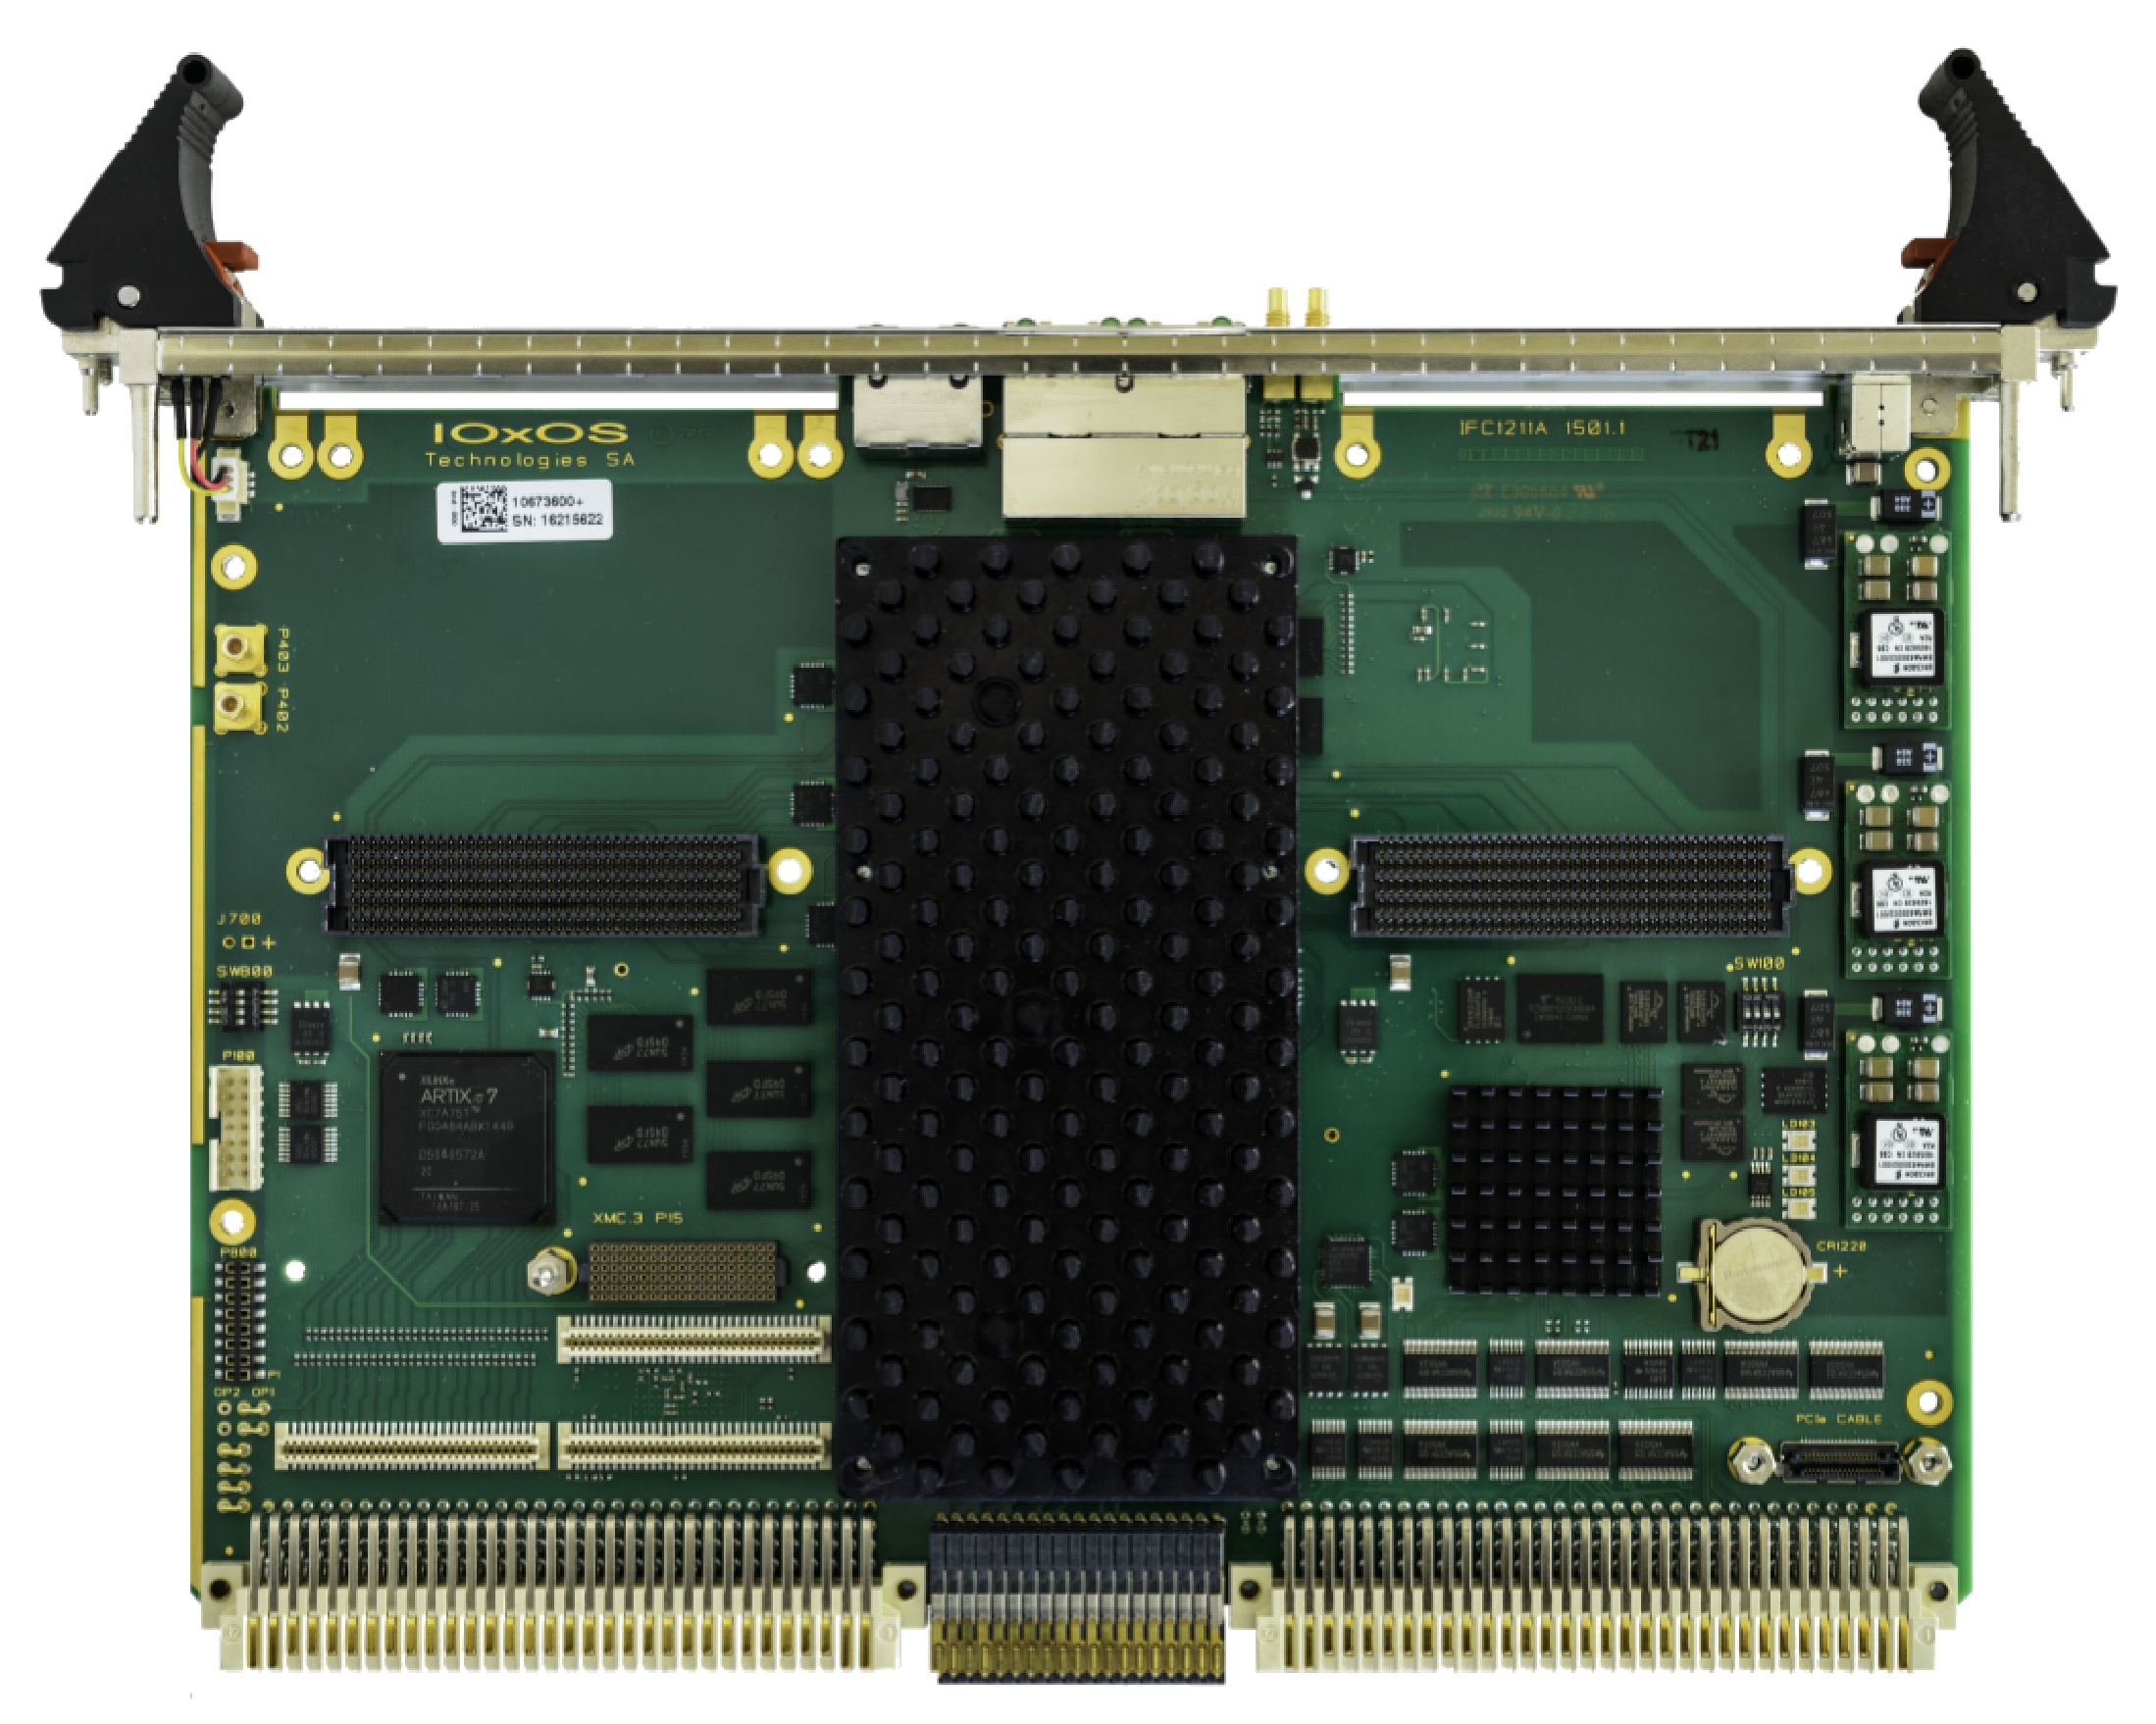
\includegraphics[width=0.80\textwidth]{./pictures/IOxOS_IFC1211.eps}
  \caption{
    IFC1211-A1 VME64x FMC Carrier with additional XMC connectors.
  }
  \label{fig:ifc1211_dim}   
\end{figure}

Figure~\ref{fig:ser_ifc_con} describes the position of the various components on the board, it is important to take note of the position of the dip switches (SWxxx) as they need to be configured before providing power to the board.

\begin{figure}[!htb]
	\centering
	\hspace*{-2.5cm}
	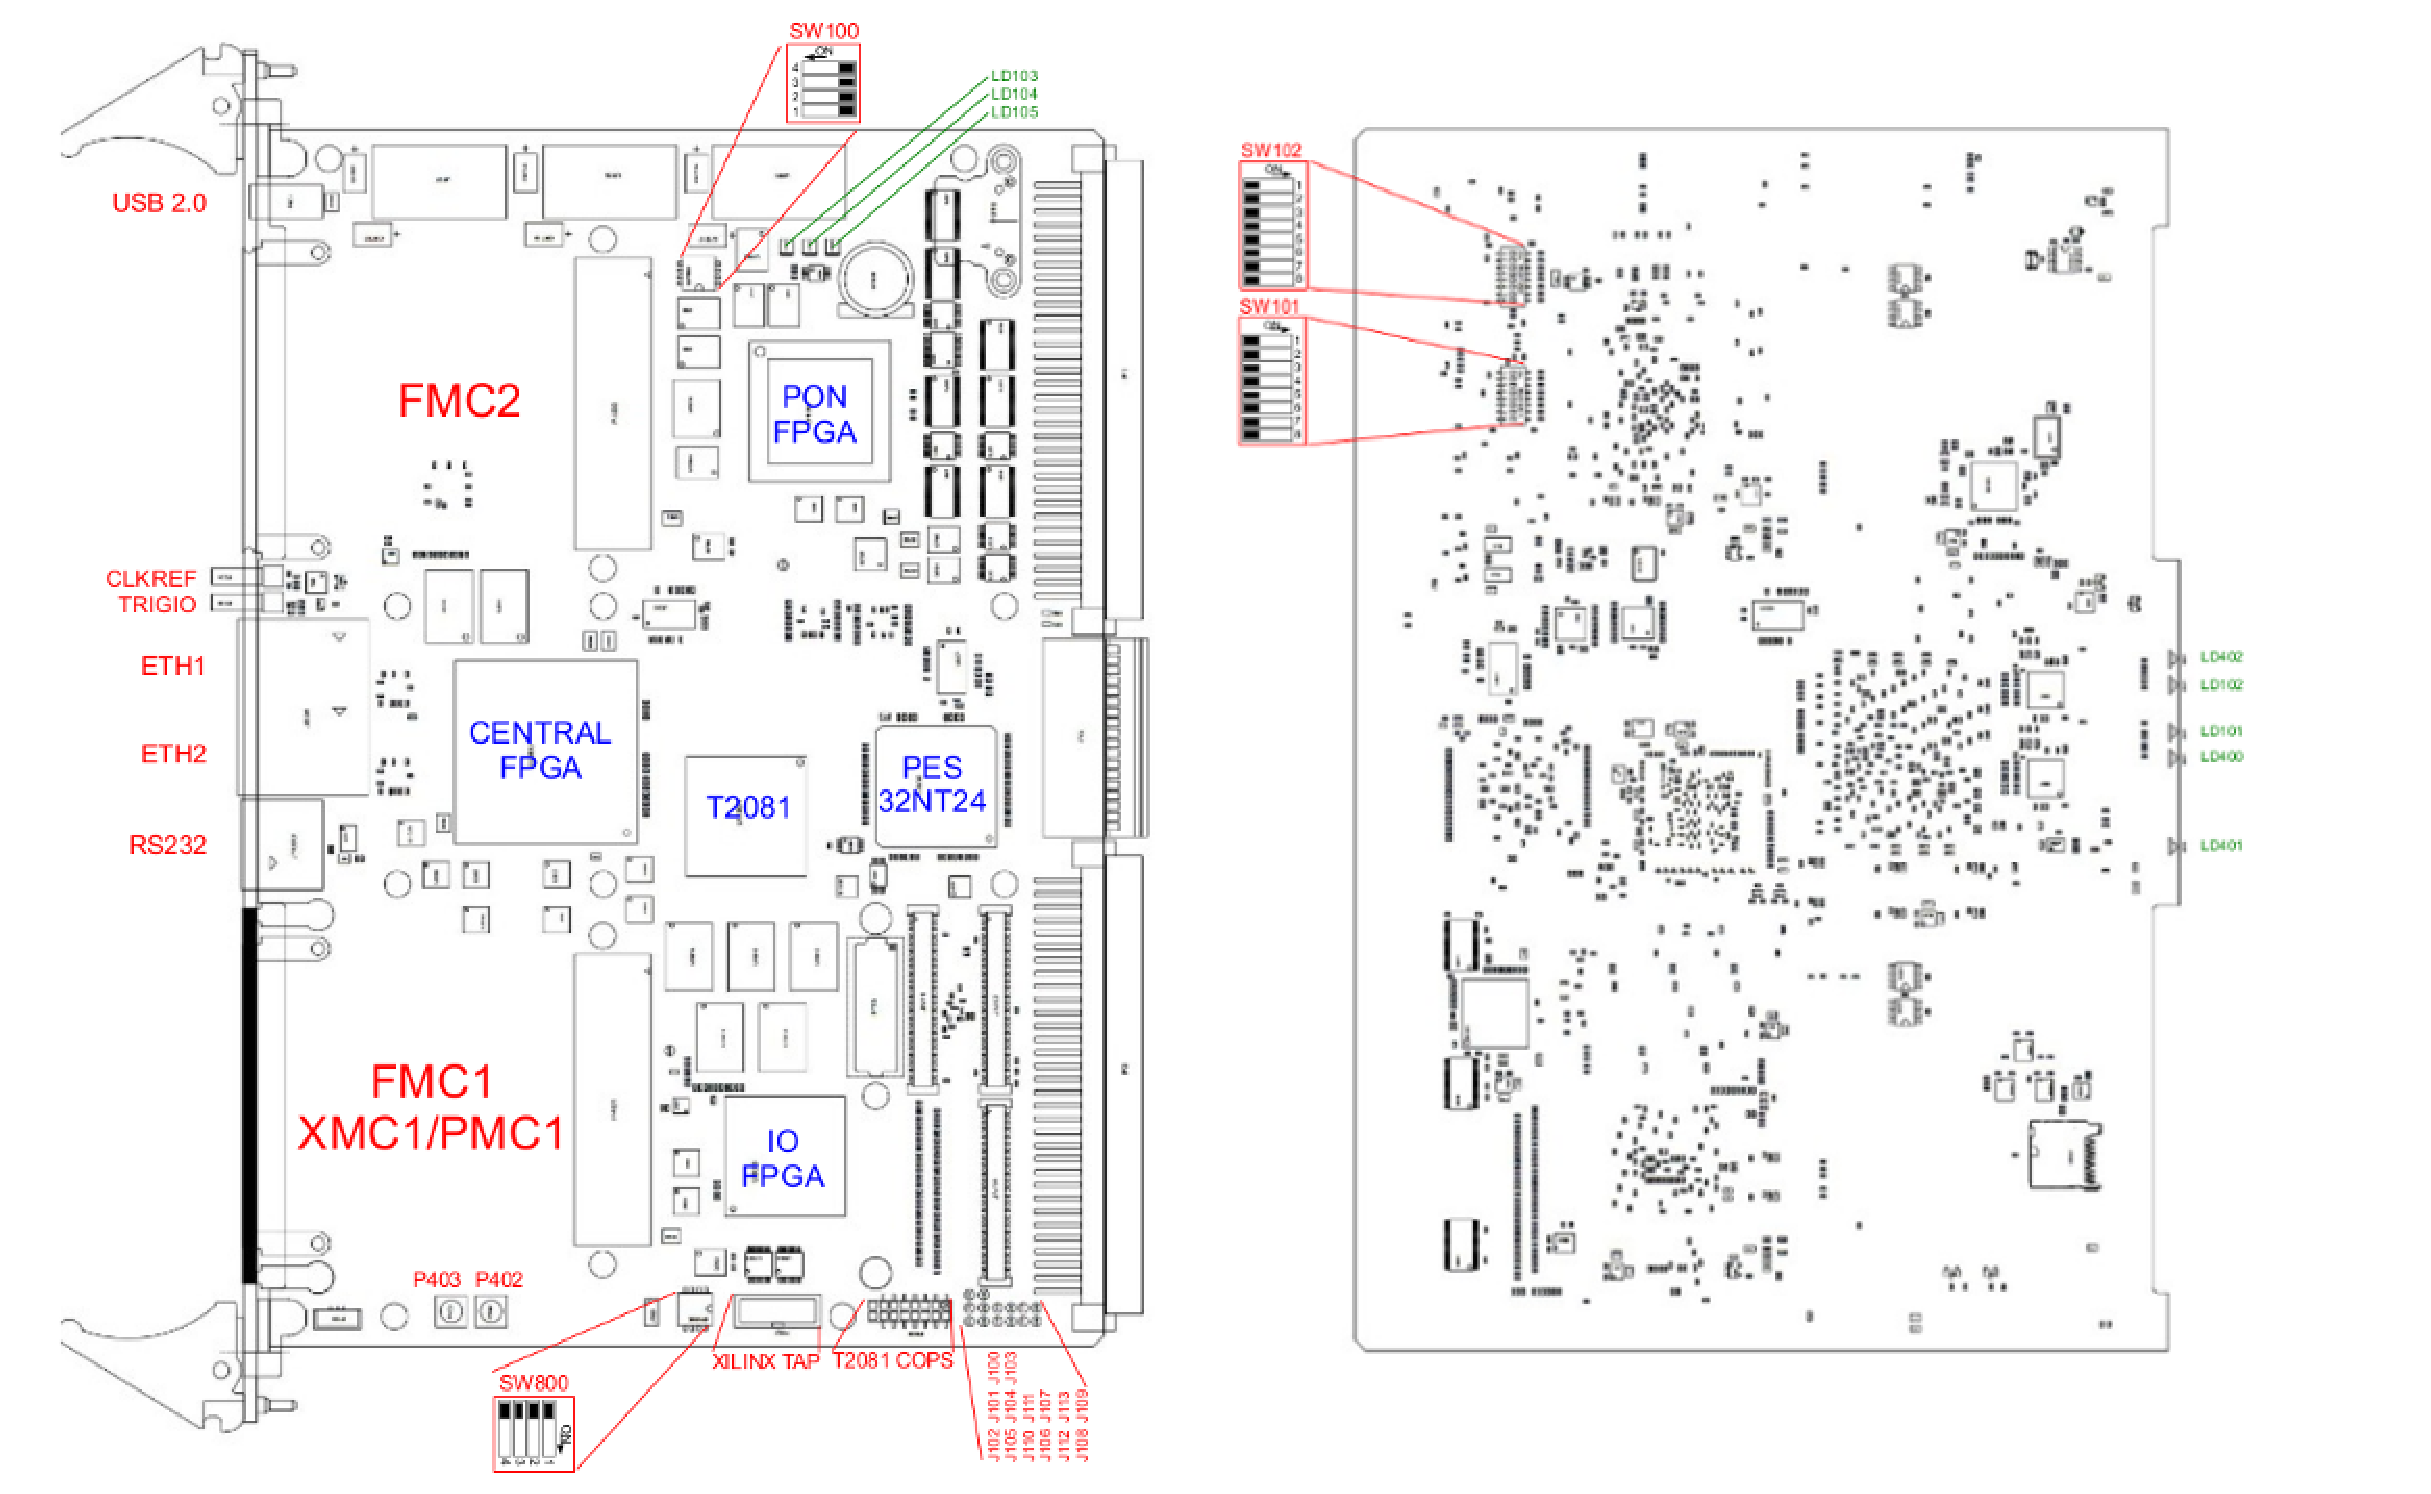
\includegraphics[width=1.4\textwidth]{./pictures/ser_ifc_con.eps}
	\caption{
		Dip Switches and Serial interface locations on the IFC1211.
	}
	\label{fig:ser_ifc_con}
\end{figure}

The block diagram shown in Figure~\ref{fig:ifc1211_bd} represents the interconnection scheme amongst the different components.

\begin{figure}[!htb]
	\centering
	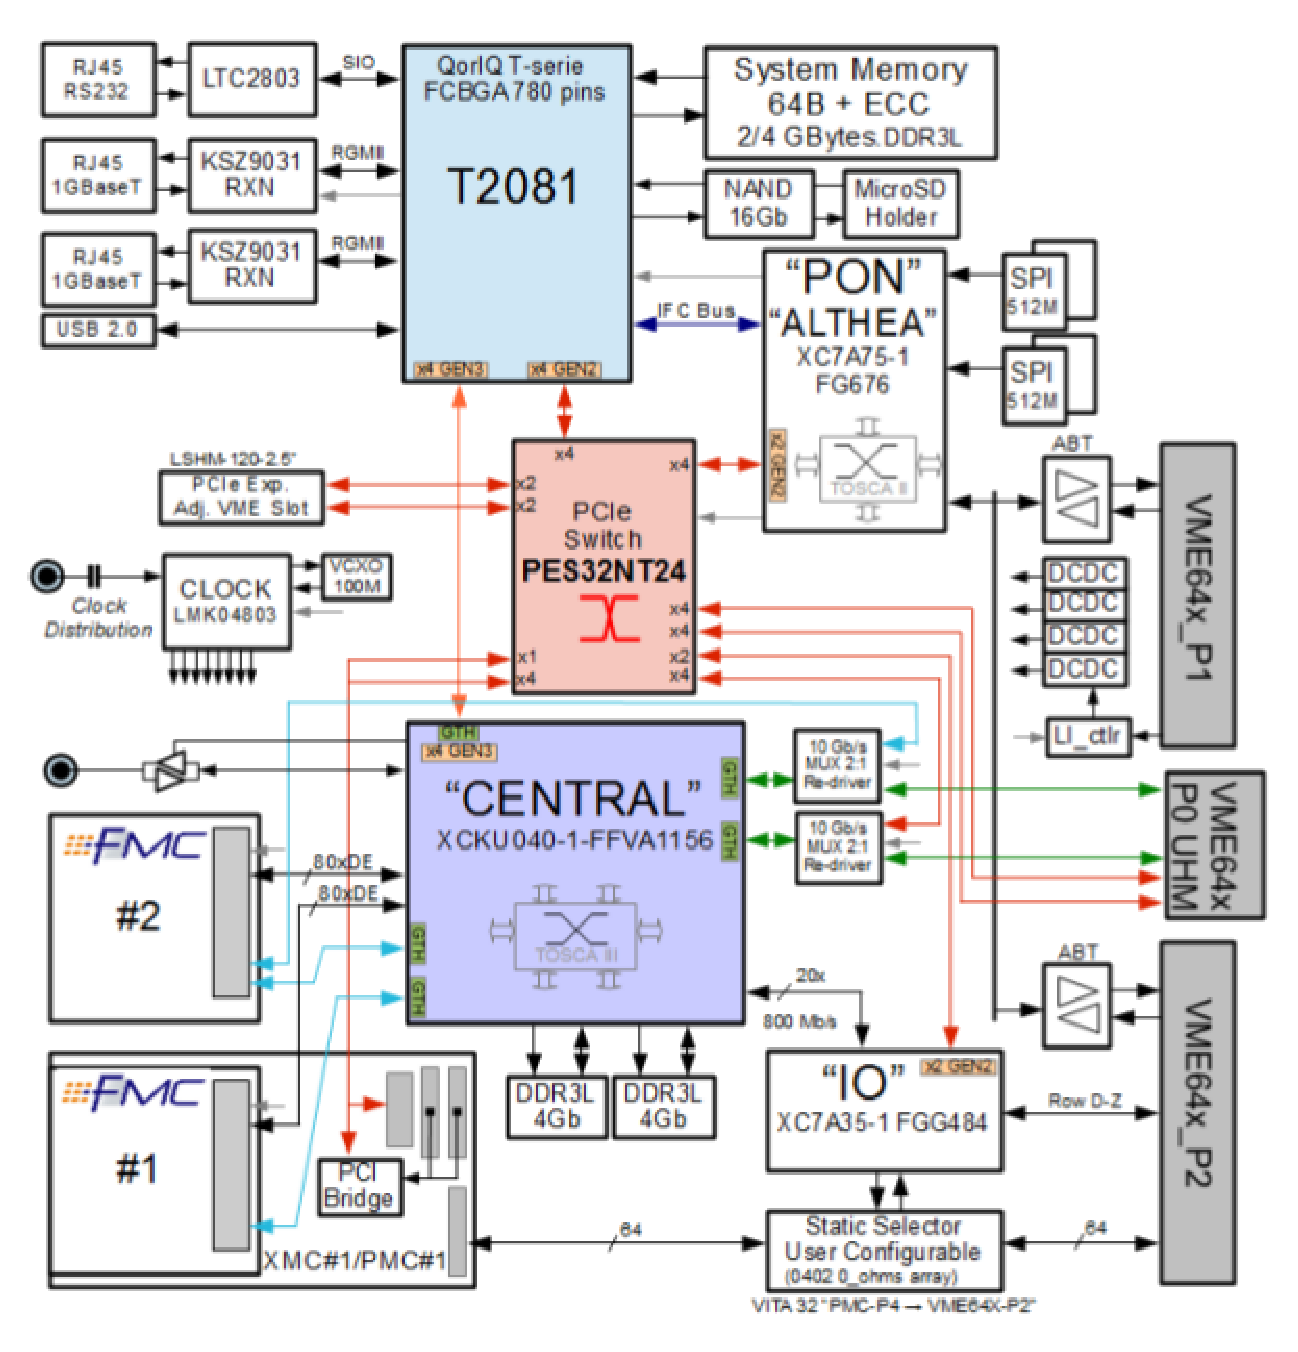
\includegraphics[width=0.80\textwidth]{./pictures/IOxOS_IFC1211_bd.eps}
	\caption{
		IFC1211-Ax VME64x Block Diagram.
	}
	\label{fig:ifc1211_bd}   
\end{figure}

As can be seen the T2081 has direct access to all the 3 front panel RJ45 connectors, two of those are actual gigabit Ethernet connections while the remaining one is a serial link.
2GBytes of DDR3-2133 memory with ECC are provided to the T2081 PowerPC processor and one additional gigabyte is made available to the Kintex Ultrascale FPGA.

The board is available in two different configurations depending on the mezzanine cards that it is supposed to host, the IFC1211-A0 version is configured to support up to two FMC HPC cards while the -A1 version is tailored for a FMC and a XMC cards.
The differential connections of both the FMCs are routed to the Xilinx Ultrascale FPGA. Additional 4 XCVR lanes per slot are provided and routed to the same FPGA MGT blocks.

%The Hardware User's Guide \cite{IFC1211_HW_TUG} also describes some added functionalities to the common U-boot distribution that allow to check and modify bitstream images for the FPGAs so that the PON FPGA can program them at startup time, all these informations are provided in the pages from 77 to 80.


\clearpage

\chapter{System Environment}
Before describing the engineering procedure necessary to boot up the IFC1211 VME board, it is necessary to have the following list of hardware and software components. Here we will show the hardware and software requirements and how to access to the infrastructure already available in the ICS lab at ESS. The information shown in this chapter is used in the ICS Lab at ESS.


\section{Hardware}
Table~\ref{table:hwlist} shows the list of hardware that is necessary to boot up the board. The hardware list provided mimics the one available in the ICS lab, if it is necessary to use a different component please be aware that despite it might provide similar functionalities it could be necessary to modify the instructions contained in this Engineering Manual according to the informations contained in the manufacturers datasheet or to the software revision number. It is assumed that a computer providing NFS and TFTP server functionalities is available and is configured properly to allow incoming connections from the IFC1211 board, if this is not the case an overview of the necessary steps is provided in the <name of document> \cite{SETUP_LAB_INFRASTRUCTURE}.

\begin{table}[!hb]
  \centering
  \begin{tabular}{l|l|l}
    \toprule
    Hardware                  & Info                                                               & Serial Number              \\\midrule
    \multicolumn{1}{l|}{\multirow{2}{*}{IFC1211}}  & \texttt{ICS TAG-382} or                       & 16370107 or                \\
    \multicolumn{1}{l|}{}     & \texttt{ICS TAG-382}                                               & 16370109                   \\\midrule
    \multicolumn{1}{l|}{\multirow{2}{*}{VME Crate}}& Hostname : icsb-vmeifc1210-529                &                            \\
    \multicolumn{1}{l|}{}     & or icsb-vmeifc1210-528                                             &                            \\\midrule
    MoxaBox                   & Hostname : ics-moxabox-01                                          &                            \\\midrule
    Serial cable              & see Figure~\ref{fig:ser_cable} and Table~\ref{table:ser_cable_tab} &                            \\\midrule
    Desktop or server PC      &                                                                    &                            \\\bottomrule
  \end{tabular}
  \caption[]{Hardware List}
  \label{table:hwlist}
\end{table}

\newpage
\subsection{IFC1211 Dip Switches Setting}
Before powering up the board it is necessary to ensure that the Dip switches whose value is read at bootstrap are configured in the right way.
The position of these switches on the board is depicted in Figure~\ref{fig:ser_ifc_con}.
Their position should be set as follows:

\begin{table}[!hb]
	\centering
	\begin{tabular}{l|l|c|c|c|c|c|c|c|c|}\hline\rowcolor{gray!30}
		\multicolumn{10}{|c|}{IFC1210 Switch setting} \\
		\hline\rowcolor{gray!10}
		\multicolumn{2}{|c|}{Switch Designator} & \multicolumn{8}{c|}{Switch Lever n$^{\circ}$} \\
		\hline
		\multicolumn{2}{|c|}{} & 1 & 2 & 3 & 4 & 5 & 6 & 7 & 8 \\
		\hline
		\multicolumn{1}{|c}{SW100} & \multicolumn{1}{c|}{:} & 0 & 0 & 0 & 0 &&&&\\\hline
		\multicolumn{1}{|c}{SW101} & \multicolumn{1}{c|}{:} & 1 & 0 & 0 & 0 & 0 & 0 & 0 & 0\\\hline
		\multicolumn{1}{|c}{SW102} & \multicolumn{1}{c|}{:} & 0 & 1 & 1 & 0 & 0 & 0 & 0 & 0\\\hline
	\end{tabular}
	\caption[]{Dip Switches Setting}
	\label{table:dp_setting}
\end{table}
\FloatBarrier


\subsection{Serial Connection}
In order to access the boot-loader shell the user shall have access to the serial interface.   
The Serial link to the IFC1211 T2081 processor is routed through a standard RJ45 connector but there is no off-the-shelf cable that matches the connection between the IFC board and the MoxaBox serial to ethernet device so the user must create his own according to the following instructions.

Figure~\ref{fig:ser_cable} shows the usual cable enumeration and Table~\ref{table:ser_cable_tab} shows the required connections at both ends assuming that the cable end at the Moxa NPort device follows the T568B coloring scheme shown.

\begin{figure}[!htb]
	\centering
	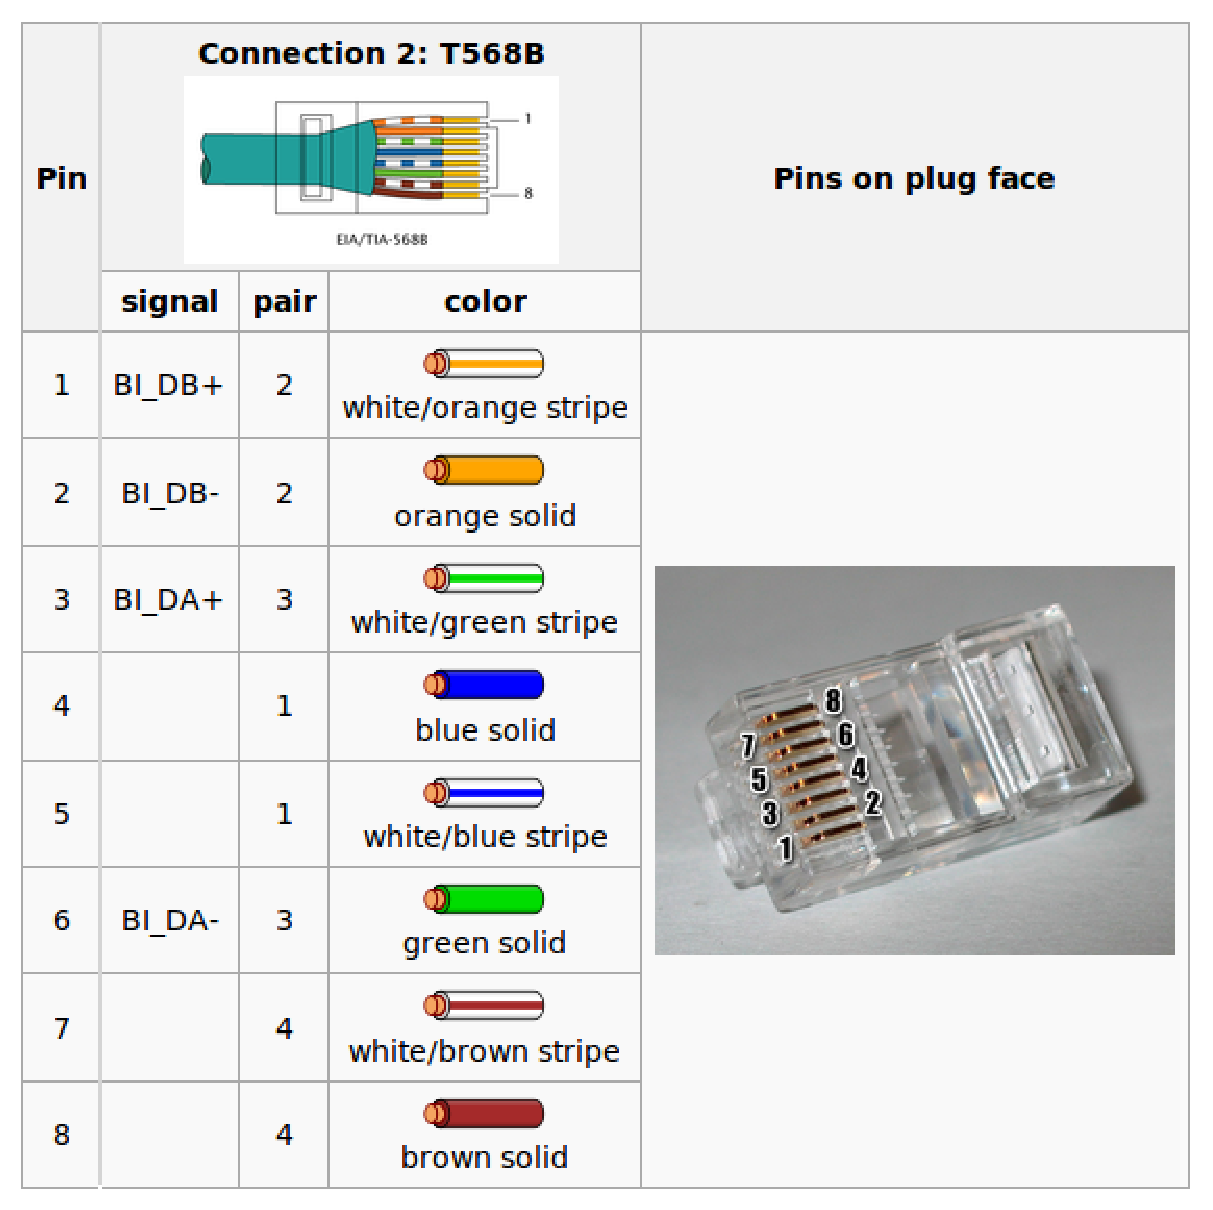
\includegraphics[width=0.80\textwidth]{./pictures/ser_cable.eps}
	\caption{
		Ethernet T568B cables enumeration.
	}
	\label{fig:ser_cable}   
\end{figure}

\begin{table}[!hb]
  \centering
  
  \begin{tabular}{|c|c|c|c|c|}\cline{2-5}
  	\multicolumn{1}{c|}{}
  	& \multicolumn{2}{c|}{\cellcolor{gray!30}\bfseries\sffamily Moxa NPort 5610 (ics-moxabox-01)} 
  	& \multicolumn{2}{c|}{\cellcolor{gray!30}\bfseries\sffamily IFC1211} \\
  	\hline
  	\cellcolor{gray!30}{\bfseries\sffamily Pin n$^{\circ}$}
  	& Color
  	& Description
  	& Color
  	& Description \\
  	\hline
  	1 & white/orange stripe & DSR (in)     & green solid                                 & Not used (DCD) \\
  	\hline\rowcolor{gray!10}%\rowcolor{LightCyan}
  	2 & orange solid        & RTS (out)    & orange solid                                & RTS            \\
  	\hline
  	3 & white/green stripe  & GND          & white/green stripe                          & GNDC           \\
  	\hline\rowcolor{gray!10}%\rowcolor{LightCyan}
  	4 & blue solid          & TxD (out)    & white/blue stripe                           & TXD            \\
  	\hline
  	5 & white/blue stripe   & RxD (in)     & blue solid                                  & RXD            \\
  	\hline\rowcolor{gray!10}%\rowcolor{LightCyan}
\iffalse
  	\multirow{2}{*}{6} & \multicolumn{1}{c|}{\multirow{2}{*}{green solid}} & \multicolumn{1}{c|}{\multirow{2}{*}{DCD (in)}} & \multicolumn{1}{c|}{none (do not connect} & \multicolumn{1}{c|}{\multirow{2}{*}{GNDC}} \\
\fi
    6 & green solid & DCD (in) & none (do not connect & GNDC \\
  	\rowcolor{gray!10}%\rowcolor{LightCyan}
  	&&&to white/orange cable)&\\
  	\hline
  	7 & white/brown stripe  & CTS (in)     & white/brown stripe                          & CTS            \\
  	\hline\rowcolor{gray!10}%\rowcolor{LightCyan}
  	8 & brown solid         & DTR (out)    & brown solid                                 & Not used (DTR) \\
  	\hline
\iffalse
  	\begin{tabular}[t]{
  			| >{\ttfamily\raggedright}p{1.0cm}
  			| >{\sffamily\raggedright}p{2.2cm}
  			| >{\sffamily}p{\dimexpr\textwidth-12\tabcolsep-0\fboxsep-9.5cm\relax} |
  		}
  		\firsthline
  		\multicolumn{1}{|l|}{\cellcolor{gray!20}\bfseries Pin n$^{\circ}$} 
  		& \multicolumn{1}{l}{\cellcolor{gray!20}\bfseries Color} 
  		& \multicolumn{1}{|l|}{\cellcolor{gray!20}\bfseries Description} \\
  		\hline
  		1 & white/orange stripe & DSR (in)   \\
  		\hline
  		2 & orange solid        & RTS (out)  \\
  		\hline
  		3 & white/green stripe  & GND        \\
  		\hline
  		4 & blue solid          & TxD (out)  \\
  		\hline
  		5 & white/blue stripe   & RxD (in)   \\
  		\hline
  		6 & green solid         & DCD (in)   \\
  		\hline
  		7 & white/brown stripe  & CTS (in)   \\
  		\hline
  		8 & brown solid         & DTR (out)  \\
  		\hline
  	\end{tabular} \\[15ex]\textbf{}
  	  &
  	\begin{tabular}[t]{
  			| >{\ttfamily\raggedright}p{1.0cm}
  			| >{\sffamily\raggedright}p{2.2cm}
  			| >{\sffamily}p{\dimexpr\textwidth-12\tabcolsep-0\fboxsep-9.5cm\relax} |
  		}
  		\firsthline
  		\multicolumn{1}{|l|}{\cellcolor{gray!20}\bfseries Pin n$^{\circ}$} 
  		& \multicolumn{1}{l|}{\cellcolor{gray!20}\bfseries Color} 
  		& \multicolumn{1}{l|}{\cellcolor{gray!20}\bfseries Description} \\
  		\hline
  		1 & green solid                                 & Not used (DCD) \\
  		\hline
  		2 & orange solid                                & RTS \\
  		\hline
  		3 & white/green stripe                          & GNDC \\
  		\hline
  		4 & white/blue stripe                           & TXD \\
  		\hline
  		5 & blue solid                                  & RXD \\
  		\hline
  		6 & none (do not connect to white/orange cable) & GNDC \\
  		\hline
  		7 & white/brown stripe                          & CTS \\
  		\hline
  		8 & brown solid                                 & Not used (DTR) \\
  		\hline
  	\end{tabular} \\[15ex]
\fi
  \end{tabular}
\iffalse
  \begin{tabular}{l|l|l}
  	\toprule
  	Pin	          & Moxa NPort 5610 (ics-moxabox-01)      & IFC1211                 \\\midrule
  	                T-568B colour	  RS-232 Signal
  \end{tabular}
\fi
\caption[]{Serial cable connections}
\label{table:ser_cable_tab}
\end{table}

The white and orange stripes cable is not routed to any pin on the IFC1211 side and is actually left dangling, in addition one of the GND pins is not connected but so far no problem was detected related to this.


\clearpage
\section{Software}
Table~\ref{table:swlist} shows the list of software and services required. It is not necessary to have the same TFTP or NFS server versions to be able to boot the IFC1211 board, but there might be a few differences in terms of their configuration.
\begin{table}[!htb]
  \centering
  \begin{tabular}{l|l}
    \toprule\rowcolor{gray!15}
    Item                      & Version and Info.                                               \\\midrule
\iffalse
    CentOS Linux              & \texttt{7.1.1503}                                               \\\midrule
    Kernel                    & \texttt{3.10.0-229.7.2.rt56.141.6.el7.centos.x86\_64}           \\\midrule
\fi
    TFTP server               & \texttt{tftp-hpa 5.2, with readline}                            \\\midrule
    NFS server                & version 3 required                                              \\\midrule
%    ics-boot-01.esss.lu.se    & boot machine with TFTP and NFS servers and cross-compiler chain \\\midrule
    uImage\_2080              & currently version \texttt{3.12}                                 \\\midrule
    t2080ifc.dtb              & N.A.                                                            \\\midrule
    root file system .tar.gz  & fsl-image-full-t2080rdb-64b.tar.gz                              \\\bottomrule
  \end{tabular}
  \caption[]{Software and its version information.}
  \label{table:swlist}
\end{table}

The file uImage\_2080 is a Linux kernel image binary file with the U-boot boot-loader wrapper. The t2080ifc.dtb is the device-tree binary file that provides informations about the available devices, their access address and the compatible drivers.
The root file system is provided as a tarball and needs to be uncompressed before it can be used, further instructions are provided later on.
An additional file named u-boot-t2080.bin might be available, this file contains the U-boot boot-loader image which should already be loaded into the flash memory of the board and as such it is not required for the tasks described in this document. If the boot-loader is not already installed or if it needs to be updated please refer to the relevant documentation.
Both TFTP and NFS services are provided by the \texttt{ics-boot-01.esss.lu.se} server located in the ICS lab.


\clearpage
\chapter{Engineering Procedure}
\iffalse
This chapter provides the minimal information necessary to configure the TFTP and NFS servers, modify the U-boot environment to allow it to load a script and to create such a compiled script file. 
\fi
This chapter provides the informations necessary to boot the IFC1211 board. The modifications required to the U-boot environment in order to automatically load a script will be described together with the steps necessary to compile such a script.
All the procedures will assume that the user have access to the \texttt{ics-boot-01.esss.lu.se} machine, available in the ics-lab network.


\iffalse
\section{TFTP Server}
The TFTP server can be installed on RedHat based distributions issuing the following command in the shell:
\begin{lstlisting}[style=termstyle]
[srvr-machine@localhost ~]$ sudo yum install tftp tftp-server* xinetd*
\end{lstlisting}

Installing the xinetd is usually also necessary.

\begin{lstlisting}[style=termstyle]
[srvr-machine@localhost ~]$ sudo yum install tftp tftp-server* xinetd*
Loaded plugins: fastestmirror, versionlock
Loading mirror speeds from cached hostfile
Resolving Dependencies
--> Running transaction check
---> Package tftp.x86_64 0:5.2-11.el7 will be installed
---> Package tftp-server.x86_64 0:5.2-11.el7 will be installed
---> Package xinetd.x86_64 2:2.3.15-12.el7 will be installed
--> Finished Dependency Resolution

Dependencies Resolved

================================================================================
Package          Arch        Version                 Repository           Size
================================================================================
Installing:
tftp             x86_64      5.2-11.el7              C7.1.1503-base       35 k
tftp-server      x86_64      5.2-11.el7              C7.1.1503-base       44 k
xinetd           x86_64      2:2.3.15-12.el7         C7.1.1503-base      128 k

Transaction Summary
================================================================================
Install  3 Packages

Total download size: 207 k
Installed size: 373 k
Is this ok [y/d/N]: y
Downloading packages:
(1/3): tftp-5.2-11.el7.x86_64.rpm                          |  35 kB   00:00     
(2/3): tftp-server-5.2-11.el7.x86_64.rpm                   |  44 kB   00:00     
(3/3): xinetd-2.3.15-12.el7.x86_64.rpm                     | 128 kB   00:00     
--------------------------------------------------------------------------------
Total                                              272 kB/s | 207 kB  00:00     
Running transaction check
Running transaction test
Transaction test succeeded
Running transaction
Installing : 2:xinetd-2.3.15-12.el7.x86_64                                1/3 
Installing : tftp-server-5.2-11.el7.x86_64                                2/3 
Installing : tftp-5.2-11.el7.x86_64                                       3/3 
Verifying  : 2:xinetd-2.3.15-12.el7.x86_64                                1/3 
Verifying  : tftp-5.2-11.el7.x86_64                                       2/3 
Verifying  : tftp-server-5.2-11.el7.x86_64                                3/3 

Installed:
tftp.x86_64 0:5.2-11.el7              tftp-server.x86_64 0:5.2-11.el7        
xinetd.x86_64 2:2.3.15-12.el7        

Complete!
\end{lstlisting}

After the installation is complete it is necessary to modify the \texttt{/etc/xinetd.d/tftp} file. The original file should look like this

\begin{lstlisting}[style=termstyle]
[srvr-machine@localhost ~]$ cat /etc/xinetd.d/tftp
# default: off
# description: The tftp server serves files using the trivial file transfer \
#	protocol.  The tftp protocol is often used to boot diskless \
#	workstations, download configuration files to network-aware printers, \
#	and to start the installation process for some operating systems.
service tftp
{
	socket_type		= dgram
	protocol		= udp
	wait			= yes
	user			= root
	server			= /usr/sbin/in.tftpd
	server_args		= -s /var/lib/tftpboot
	disable			= yes
	per_source		= 11
	cps			= 100 2
	flags			= IPv4
}
\end{lstlisting}

and the fields "server_args" and "disable" shall be replaced with 

\begin{lstlisting}[style=termstyle]
	server_args		= -p -svv /export
	disable			= no
\end{lstlisting}

The folder in "server_args" is not mandatory to be defined to be "/export" but it might be any user-defined path existing in the machine. The remaining of the document will continue to use the previously defined folder so, if it is necessary to change it, care must be taken to modify it in all the files to reflect its new value.

Before being able start the TFTP server automatically at boot time the "/usr/lib/systemd/system/tftp.service" file has to be modified with the addition of the section \texttt{[Install]}. The modified file should look like this.

\begin{lstlisting}[style=termstyle]
[srvr-machine@localhost ~]$ cat /usr/lib/systemd/system/tftp.service 
[Unit]
Description=Tftp Server

[Service]
ExecStart=/usr/sbin/in.tftpd -p -svv /export
StandardInput=socket

[Install]
WantedBy=multi-user.target
\end{lstlisting}

Now that the previous file has been modified the TFTP server can be set to automatically start after boot by means of the following commands. Please note that you need to be root in order for the command to run successfully.

\begin{lstlisting}[style=termstyle]
[root@localhost ~]# systemctl enable xinetd
[root@localhost ~]# systemctl enable tftp
\end{lstlisting}

There is no need to add write support from the IFC1211 to the server PC so we do not need to modify the SELinux configuration.
The TFTP server should be up and running now but still no external machine should be able to access it. This is related to \texttt{firewalld} settings. 
The first command below allows clients to access the port connected to the TFTP service, but to this setting to be effective it is also necessary to issue the second one that reloads the firewalld configuration.

\begin{lstlisting}[style=termstyle]
[srvr-machine@localhost ~] sudo firewall-cmd --zone=public --add-service=tftp --permanent
...
[srvr-machine@localhost ~] sudo firewall-cmd --reload
\end{lstlisting}


\section{NFS Server}
\fi

\section{U-boot Script File}
The U-boot script file is used to modify the boot loader environment variables in order to define the booting procedure of the system.

\subsection{Default Environment and System Access}
It might be useful to take a look at the default environment settings of a system before editing them. To be able to access the U-boot shell we need to connect to the serial interface of the IFC1211 through the MoxaBox (Hostname : ics-moxabox-01 in the ics-lab network) using the cable previously defined in this document.

Figure~\ref{fig:ser_ifc_con} shows the location of the serial interface on the IFC1211 board.

Configure an available MoxaBox port according to the following values:

\begin{table}[!htb]
	\centering
	\begin{tabular}{l|l}
		\toprule\rowcolor{gray!15}
		Parameter          & Value                        \\\midrule
		Baud rate          & 155200                       \\\midrule
		Data bits          & 8                            \\\midrule
		Stop bits          & 1                            \\\midrule
		Parity             & None                         \\\midrule
		Flow control       & None                         \\\midrule
		FIFO               & Enable                       \\\midrule
		Interface          & RS-232 Only                  \\\bottomrule
	\end{tabular}
	\caption[]{MoxaBox port configuration}
	\label{table:moxa_serial}
\end{table}

To do so open a web browser and access the \texttt{http://10.4.3.90/}, under ``Serial Settings'' choose the appropriate port number and modify the values to reflect the IFC1211 settings previosly described.
Connect the appropriate end of the Ethernet cable to the IFC1211 and to the configured port on the MoxaBox.
The driver required to interface to the MoxaBox is already installed on the \texttt{ics-workstation (10.4.3.18)}, if you need to setup the communication to this device on your pc the relevant informations are described in the ESS wiki in the ``How To Setup Serial Communication to Moxa NPort 5610 on Your Machine'' section of the \cite{ASDLL} document.
To communicate with the serial interface of the device ssh into the \texttt{ics-workstation} and use the picocom tool, remember that the port enumeration in Linux starts from 0 so the \texttt{ttyr} number is the port number written on the MoxaBox chassis minus one.
\begin{lstlisting}[style=termstyle]
[srvr-machine@localhost ~]$ picocom -b 115200 /dev/ttyr1
\end{lstlisting}
The \texttt{-b} option allows to specify the baudrate of the connection if it needs be.

The U-boot shell should now be displayed and the \texttt{printenv} command will return the environment variables used at boot time. Here follows the default environment setting for the IFC1211 connected on port number 9 of the MoxaBox.

\begin{lstlisting}[style=termstyle]
[srvr-machine@localhost ~]$ picocom -b 115200 /dev/ttyr8
picocom v1.7

port is        : /dev/ttyr8
flowcontrol    : none
baudrate is    : 115200
parity is      : none
databits are   : 8
escape is      : C-a
local echo is  : no
noinit is      : no
noreset is     : no
nolock is      : no
send_cmd is    : sz -vv
receive_cmd is : rz -vv
imap is        : 
omap is        : 
emap is        : crcrlf,delbs,

Terminal ready

=> 
=> printenv
baudrate=115200
bdev=sda3
bootargs=root=/dev/ram rw console=ttyS0,115200
bootcmd=setenv bootargs root=/dev/ram rw console=$consoledev,$baudrate $othbootargs;setenv ramdiskaddr 0x02000000;setenv fdtaddr 0x00c00000;setenv loadaddr 0x1000000;bootm $loadaddr $ramdiskaddr $fdtaddr
bootdelay=-1
bootfile=images/ifc1211-default/uImage_ifc1211-201610111554.bin
consoledev=ttyS0
eth1addr=7c:dd:20:10:01:13
ethact=FM1@DTSEC4
ethaddr=7c:dd:20:10:01:12
ethprime=FM1@DTSEC4
fdtaddr=2000000
fdtfile=images/ifc1211-default/t2080ifc.dtb
fileaddr=2000000
filesize=8baf
fman_ucode=eff00000
gatewayip=10.4.0.1
hostname=IFC1211_101
hwconfig=fsl_ddr:ctlr_intlv=cacheline,bank_intlv=auto;usb1:dr_mode=host,phy_type=utmi
ipaddr=192.168.1.138
loadaddr=1000000
netdev=eth1
netmask=255.255.252.0
nfsboot=setenv bootargs root=/dev/nfs rw nfsroot=$serverip:$rootpath ip=$ipaddr:$serverip:$gatewayip:$netmask:$hostname:$netdev:off console=$consoledev,$baudrate $othbootargs;tftp $loadaddr $bootfile;tftp $fdtaddr $fdtfile;bootm $loadaddr - $fdtaddr
ramboot=setenv bootargs root=/dev/ram rw console=$consoledev,$baudrate $othbootargs;tftp $ramdiskaddr $ramdiskfile;tftp $loadaddr $bootfile;tftp $fdtaddr $fdtfile;bootm $loadaddr $ramdiskaddr $fdtaddr
ramdiskaddr=5000000
ramdiskfile=ramdisk.uboot
rootpath=/data/T2081/rootfs_2080_1.9
serverip=194.47.240.7
stderr=serial
stdin=serial
stdout=serial
tftpflash=tftpboot $loadaddr $uboot && protect off $ubootaddr +$filesize && erase $ubootaddr +$filesize && cp.b $loadaddr $ubootaddr $filesize && protect on $ubootaddr +$filesize && cmp.b $loadaddr $ubootaddr $filesize
uboot=u-boot-t2080.bin
ubootaddr=0xeff40000

Environment size: 1702/8188 bytes
=> 
\end{lstlisting}

This default environment does not allow the user to load a U-boot script at startup, in order to be able to do so the user needs to modify it. The following sections will describe how to configure the boot loader to load a script file but before that the procedure to create the script itself will be covered.


\subsection{U-boot Script Creation and Compilation}
The U-boot script is just a plain text file that will afterwards be compiled in order to be recognized by the boot loader, as such it can be created using any text editor and does not need to have any specific file extension.
To avoid any misunderstanding we will append the extension .scr on the compiled script and .script on the regular text file.
The script can contain any command that could also be issued in the boot loader shell, to view the list available commands enter \texttt{help} or \texttt{?} in the shell.

\begin{lstlisting}[style=termstyle]
=>
=> ?
?       - alias for 'help'
base    - print or set address offset
bdinfo  - print Board Info structure
boot    - boot default, i.e., run 'bootcmd'
bootd   - boot default, i.e., run 'bootcmd'
bootelf - Boot from an ELF image in memory
bootm   - boot application image from memory
bootp   - boot image via network using BOOTP/TFTP protocol
bootvx  - Boot vxWorks from an ELF image
chpart  - change active partition
cmp     - memory compare
conf    - Board configuration
coninfo - print console devices and information
cp      - memory copy
cpld    - Reset the board or alternate bank
cpu     - Multiprocessor CPU boot manipulation and release
crc32   - checksum calculation
date    - get/set/reset date & time
dhcp    - boot image via network using DHCP/TFTP protocol
echo    - echo args to console
editenv - edit environment variable
env     - environment handling commands
erase   - erase FLASH memory
errata  - Report errata workarounds
exit    - exit script
ext2load- load binary file from a Ext2 filesystem
ext2ls  - list files in a directory (default /)
false   - do nothing, unsuccessfully
fatinfo - print information about filesystem
fatload - load binary file from a dos filesystem
fatls   - list files in a directory (default /)
fatsize - determine a file's size
fdt     - flattened device tree utility commands
flinfo  - print FLASH memory information
fpga    - access FPGA(s)
go      - start application at address 'addr'
hash    - compute hash message digest
help    - print command description/usage
i2c     - I2C sub-system
iminfo  - print header information for application image
imls    - list all images found in flash
imxtract- extract a part of a multi-image
itest   - return true/false on integer compare
loadb   - load binary file over serial line (kermit mode)
loads   - load S-Record file over serial line
loadx   - load binary file over serial line (xmodem mode)
loady   - load binary file over serial line (ymodem mode)
loop    - infinite loop on address range
mac     - display and program the system ID and MAC addresses in EEPROM
md      - memory display
mdio    - MDIO utility commands
mii     - MII utility commands
mm      - memory modify (auto-incrementing address)
mmc     - MMC sub system
mmcinfo - display MMC info
mtdparts- define flash/nand partitions
mtest   - simple RAM read/write test
mw      - memory write (fill)
nand    - NAND sub-system
nboot   - boot from NAND device
nfs     - boot image via network using NFS protocol
nm      - memory modify (constant address)
pci     - list and access PCI Configuration Space
ping    - send ICMP ECHO_REQUEST to network host
printenv- print environment variables
prom    - PROM handling
protect - enable or disable FLASH write protection
reginfo - print register information
reset   - Perform RESET of the CPU
run     - run commands in an environment variable
sata    - SATA sub system
saveenv - save environment variables to persistent storage
setenv  - set environment variables
setexpr - set environment variable as the result of eval expression
sf      - SPI flash sub-system
showvar - print local hushshell variables
sleep   - delay execution for some time
source  - run script from memory
test    - minimal test like /bin/sh
tftpboot- boot image via network using TFTP protocol
true    - do nothing, successfully
usb     - USB sub-system
usbboot - boot from USB device
vdd_override- override VDD
vdd_read- read VDD
version - print monitor, compiler and linker version
=>
\end{lstlisting}

In order to be able to boot up the IFC1211 we need to define its network settings, specify the necessary files locations and also provide some basic boot arguments.
The files required are:
\begin{itemize}
	\item uImage\_2080, the linux kernel image;
	\item t2080ifc.dtb, the compiled device tree binary;
	\item fsl-image-full-t2080rdb-64b.tar.gz, the root file system structure (this file needs to be extracted).
\end{itemize}
In addition the following FPGA bitstream files can be loaded at startup and should be also provided:
\begin{itemize}
	\item io.bit, the IO FPGA bitstream configuration file;
	\item central.bit, the CENTRAL FPGA bitstream configuration file.
\end{itemize}
These files need to be copied to the export directory of any available server providing TFTP and NFS functionalities.
The \texttt{ics-boot-01.esss.lu.se} machine provides all these services, its export directory is \texttt{/export} and its directory structure is as follows
\begin{lstlisting}[style=termstyle]
[username@ics-boot-01 export]$ tree -d -L 2
.
├── boot
│   ├── EFI
│   ├── images
│   └── pxelinux.cfg
├── epics
│   ├── bases
│   └── modules
├── images
│   ├── ifc1210-default
│   ├── ifc1210-maurizio
│   ├── ifc1210-rflps
│   ├── ifc1210-scope
│   ├── ifc1211-default
│   └── mtcacpu-default
├── modules
│   └── centos7
├── nfsroots
│   ├── centos7
│   ├── ifc1210
│   └── ifc1211
├── sandbox
│   ├── bases
│   └── modules
├── sb-startup
│   └── ioc
├── sdk
│   └── eldk-5.6
└── startup
├── boot
└── ioc
\end{lstlisting}

To keep the files organized copy the \texttt{uImage\_2080} and \texttt{t2080ifc.dtb} files into the \texttt{images/ifc1211-default} folder and untar the root file system in \texttt{nfsroots/ifc1211}.
Copy the io.bit and central.bit files to the \texttt{images/ifc1211-default} folder if they are available.
We are now ready to define the content of the U-boot script which should be as follows:

\begin{lstlisting}[style=texteditor]
setenv fpgaIO /images/ifc1211-default/io.bit
setenv fpgaCE /images/ifc1211-default/central.bit
setenv bootfile images/ifc1211-default/uImage_2080
setenv fdtfile images/ifc1211-default/t2080ifc.dtb
setenv serverip 194.47.240.7
setenv rootpath /export/nfsroots/ifc1211/rootfs
setenv nfsver nfsvers=3
setenv ipaddr 10.4.3.28
setenv gatewayip 10.4.0.1
setenv netmask 255.255.252.0
setenv hostname IFC1211_101
setenv netdev eth0
setenv consoledev ttyS0
setenv baudrate 115200
setenv othbootargs rootdelay=1 earlyprintk
setenv bootargs root=/dev/nfs nfsroot=$serverip:$rootpath,$nfsver ip=$ipaddr:$serverip:$gatewayip:$netmask:$hostname:$netdev:off console=$consoledev,$baudrate $othbootargs ramdisk=60000 pci_scan_all pci=realloc
setenv nfsboot 'setenv bootargs $bootargs;tftp $loadaddr $bootfile;tftp $fdtaddr $fdtfile;bootm $loadaddr - $fdtaddr'
setenv loadIO 'tftp $loadaddr $fpgaIO;fpga load io $loadaddr'
setenv loadCE 'tftp $loadaddr $fpgaCE;fpga load central $loadaddr'
setenv fpgaload 'run loadIO; run loadCE; fpga reset 11b01'
\end{lstlisting}

The first two lines and the last three are optional and should be included only if the bitstream files have been provided.
This file will not be recognized by U-boot unless we translate it to a proper script, in order to do this copy it to any folder in the \texttt{ics-boot-01.esss.lu.se} machine where the user has writing privileges, here it is assumed to be the user home directory, and issue the following command:

\begin{lstlisting}[style=termstyle]
[username@ics-boot-01 ~]$ /home/shared/SVN/Software/IOxOS/u-boot/setenv/mkimage -T script -C none -n 'Boot Script' -d uboot_ifc1211.script uboot_ifc1211.scr
\end{lstlisting}

where \texttt{\_ifc1211} is supposed to be the name of text file created in the previous step and also the desired name for the compiled script.

If the mkimage executable is not available in the location shown above a way to find it is to run the following command.

\begin{lstlisting}[style=termstyle]
[username@ics-boot-01 ~]$ find / ! -readable -prune -o -path *u-boot* -name mkimage -print
\end{lstlisting}

This will display all available files named \texttt{mkimage} that are located in a folder with \texttt{u-boot} in its path.

The generated \texttt{.scr} file has to be copied in the \texttt{/export} folder in order to be retrieved by U-boot using the TFTP service, in the remainder of the document it will be assumed that this file has been copied in \texttt{/export/boot}.



\subsection{U-boot environment setup to load script}
The generated script is now ready to be retrieved and loaded from the server.
The user must instruct U-boot to load the file and this is done by modifying the default Environment.
Connect to the IFC1211 board serial interface, as described previously, and type the following commands:

\begin{lstlisting}[style=termstyle]
[srvr-machine@localhost ~]$ picocom -b 115200 /dev/ttyr8
picocom v1.7

port is        : /dev/ttyr8
flowcontrol    : none
baudrate is    : 115200
parity is      : none
databits are   : 8
escape is      : C-a
local echo is  : no
noinit is      : no
noreset is     : no
nolock is      : no
send_cmd is    : sz -vv
receive_cmd is : rz -vv
imap is        : 
omap is        : 
emap is        : crcrlf,delbs,

Terminal ready

=> setenv bootcmd 'run envload'
=> setenv envload 'if tftp $loadaddr $serverip:boot/env-$eth1addr.scr; then source $loadaddr && run fpgaload && run nfsboot; elif tftp $loadaddr $serverip:boot/uboot_ifc1211.scr; then source $loadaddr && run fpgaload && run nfsboot; else false; fi'
=> saveenv
\end{lstlisting}

The \texttt{envload} instruction translates to the following list of actions:

\begin{itemize}
	\item if a file named env-\$eth1addr.scr is found on the server and can be loaded at the \$loadaddr address in memory then:
	\begin{itemize}
		\item source the address where the file was copied, which means to import and to execute the contained instructions;
		\item run the instruction called \texttt{fpgaload};
		\item run the instruction called \texttt{nfsboot};
	\end{itemize}
	\item otherwise if a file named uboot\_ifc1211.scr is found on the server and can be loaded at the \$loadaddr address in memory then:
	\begin{itemize}
		\item source the address where the file was copied, which means to import and to execute the contained instructions;
		\item run the instruction called \texttt{fpgaload};
		\item run the instruction called \texttt{nfsboot};
	\end{itemize}
	\item otherwise if none of the previous two conditions apply do nothing.
\end{itemize}

The \texttt{\$loadaddr} variable is defined in the default U-boot environment and translates to a memory address.
The \texttt{env-\$eth1addr.scr} is introduced to reflect what the default naming scheme will look like when deploying the boards in the facility and translates to a file name that includes the MAC address of the network interface \texttt{eth1}, in this way any script file will be associated only to a board.
If the bitstream files are not available the instruction \texttt{\&\& run fpgaload} shall be removed from the previous command.
The IFC1211 can now be booted up by issuing the \texttt{boot} command in the U-boot shell at every startup, to avoid the necessity to interact with the board every time it resets or power cycles the following additional modification can be made to the environment: 

\begin{lstlisting}[style=termstyle]
[srvr-machine@localhost ~]$ picocom -b 115200 /dev/ttyr8
picocom v1.7

port is        : /dev/ttyr8
flowcontrol    : none
baudrate is    : 115200
parity is      : none
databits are   : 8
escape is      : C-a
local echo is  : no
noinit is      : no
noreset is     : no
nolock is      : no
send_cmd is    : sz -vv
receive_cmd is : rz -vv
imap is        : 
omap is        : 
emap is        : crcrlf,delbs,

Terminal ready

=> setenv bootdelay 5
=> saveenv
\end{lstlisting}

This will make U-boot wait for 5 second at every startup to see if the user wants to stop the booting procedure otherwise it will run the boot command.



\clearpage
\backmatter
%\bibliographystyle{unsrt}
%\bibliographystyle{plainnat}
%\bibliographystyle{abbrvnat}
\bibliographystyle{unsrtnat}
%\bibliographystyle{chicago}
\bibliography{./ess_refs}

\end{document}



%% The output of \verb|lspci| for the PCIe-EVR-300 is:
%% \begin{lstlisting}
%% $ lspci -s 05:00 -vv
%% 05:00.0 Signal processing controller: Lattice Semiconductor Corporation Device
%%         ec30 (rev 01)
%%     Subsystem: Device 1a3e:172c
%%     Control: I/O+ Mem+ BusMaster+ SpecCycle- MemWINV- VGASnoop- ParErr-
%%         Stepping- SERR- FastB2B- DisINTx-
%%     Status: Cap+ 66MHz- UDF- FastB2B- ParErr- DEVSEL=fast >TAbort- <TAbort-
%%         <MAbort- >SERR- <PERR- INTx-
%%     Latency: 0, Cache Line Size: 64 bytes
%%     Interrupt: pin A routed to IRQ 16
%%     Region 0: Memory at c0400000 (32-bit, non-prefetchable) [size=1M]
%%     Capabilities: <access denied>
%%     Kernel driver in use: mrf-pci

%% $ lspci -s 05:00 -t
%% -+-[0000:05]---00.0
%%  \-[0000:00]-
%% \end{lstlisting}




%% \chapter{Requirements}

%% \section{FAI Server}
%% The most works will be done in so-called a faiserver, as a typical PC. We uses Debian 7 Wheezy up-to-date version as OS and its system information (\texttt{uname -a} is as follows:
%% \begin{lstlisting}
%% Linux faiserver 3.2.0-4-amd64 #1 SMP Debian 3.2.57-3+deb7u1 x86_64 GNU/Linux
%% \end{lstlisting}

%% \section{Media Access Control (MAC) addresses of Target Computers}
%% We need to get MAC address of target PCs. Here we use two PCs : one is the real PC, and another is the virtual one by vmplayer. The real one is named as \textit{demohost} and the virtual one does \textit{gnomehost}. Two names are simply used by using the fai-example configuration. So the total computers are \textbf{faiserver}, \textbf{demohost}, and \textbf{gnomehost}. Figure~\ref{fig:vmplayer_network} shows the vmplayer screen-shot of the MAC address for a virtual PC.

%% For the installation examples, two MAC addresses and the hostnames are used as follows :
%% \begin{itemize}
%% \item demohost  : \texttt{E8:03:9A:63:83:81}
%% \item gnomehost : \texttt{00:50:56:39:D9:1E}
%% \end{itemize}
%% \begin{figure}[!htb]
%%   \centering
%%   \includegraphics[width=0.96\textwidth]{./images/vmplayer_network.eps}
%%   \caption{
%%             MAC address setup for a virtual PC by using vmplayer.
%%           }
%%   \label{fig:vmplayer_network}   
%% \end{figure}

%% %%  Get MAC address on target PC (demohost, gnomehost)
%% %%   - VMWare Host : Network Bridget, Generate MAC address, use it in /etc/dhcp/dhcpd.conf
%% %%   - real   Host : Get MAC address...

%% \clearpage

%% \section{Packages}
%% We will use the up-to-date fai packages from fai-project site\footnote{\url{http://fai-project.org}} instead of the Debian Wheezy repository. The first thing is to modify the apt sources list to let the system know where the fai project is

%% \begin{lstlisting}%[caption={Modify the apt source list}]

%% root@faiserver:~# emacs /etc/apt/sources.list

%%   deb http://ftp.lecl.net/debian/ wheezy main contrib non-free
%%   deb http://fai-project.org/download wheezy koeln

%% root@faiserver:~# aptitude update

%% \end{lstlisting}

%% The next step is to install the fai packages such as \texttt{fai-client}, \texttt{fai-server}, and \texttt{fai\-quickstart}. Debian will care the other package dependencies, so simply use the following command : 

%% \begin{lstlisting}%[caption={Installation of \texttt{fai-client}, \texttt{fai-server}, and \texttt{fai-quickstart}}]

%% root@faiserver:/etc# aptitude install fai-client fai-server fai-quickstart

%% The following NEW packages will be installed:
%%   debootstrap{a} fai-client fai-doc{a} fai-quickstart fai-server libapt-pkg-perl{a} libgraph-perl{a} libheap-perl{a} 
%%   libproc-daemon-perl{a} libproc-processtable-perl{a} nfs-kernel-server{a} openbsd-inetd{a} reprepro{a} 
%% 0 packages upgraded, 13 newly installed, 0 to remove and 0 not upgraded.
%% Need to get 0 B/2,137 kB of archives. After unpacking 4,829 kB will be used.
%% Do you want to continue? [Y/n/?] 

%% ......................................
%% ......................................


%% Setting up nfs-kernel-server (1:1.2.6-4) ...
%% [ ok ] Stopping NFS kernel daemon: mountd nfsd.
%% [ ok ] Unexporting directories for NFS kernel daemon....
%% [warn] Not starting NFS kernel daemon: no exports. ... (warning).
%% Setting up openbsd-inetd (0.20091229-2) ...
%% [ ok ] Stopping internet superserver: inetd.
%% [info] Not starting internet superserver: no services enabled.
%% Setting up debootstrap (1.0.48+deb7u1) ...
%% Setting up fai-client (4.2) ...
%% Setting up fai-doc (4.2) ...
%% Setting up fai-server (4.2) ...
%% You might want to edit fai.conf and nfsroot.conf in /etc/fai or
%% go with the defaults. You should edit /etc/fai/apt/sources.list
%% for faster access to a package repository.
%% Setting up reprepro (4.12.5-1) ...
%% Setting up fai-quickstart (4.2) ...

%% \end{lstlisting}


%% \section{Dynamic Host Configuration Protocol (DHCP) Configuration}
%% The DHCP setting has all FAI host computers' MAC address and its ip address. And if there is no isc-dhcp packages, please install them by using the following command:
%% \begin{lstlisting}
%% root@faiserver:~# aptitude install isc-dhcp-server
%% \end{lstlisting}
%% Since the DHCP configuration is essential for the FAI setup, please edit dhcp daemon configuration file (dhcpd.conf) as follows:

%% \begin{lstlisting}
%% root@faiserver:/etc# emacs /etc/dhcp/dhcpd.conf
%% \end{lstlisting}
%% The following example is used in the \texttt{10.1.4.0} subnet inside the RISP 2nd floor office network. So, the ip range is limited for only two addresses (210 and 211). The \texttt{domain-name} is provided by the local nameserver (\texttt{10.1.5.11}). The gateway of the \texttt{10.1.4.0} subnet is used as \texttt{routers}. The DHCP server has \texttt{10.1.4.100}.

%% \begin{lstlisting}
%% ddns-update-style none;
%% log-facility local7;

%% deny unknown-clients;
%% option dhcp-max-message-size 2048;
%% use-host-decl-names on;

%% subnet 10.1.4.0 netmask 255.255.255.0 {

%%        option domain-name         "risp.invalid";
%%        option domain-name-servers 10.1.5.11;
%%        option routers             10.1.4.254;

%%        range  10.1.4.210 10.1.4.211;
%%        default-lease-time 60;
%%        max-lease-time 720;

%%        next-server 10.1.4.100;
%%        filename "fai/pxelinux.0";
%% }

%% host demohost {
%%         hardware ethernet e8:03:9a:63:83:81;
%%         fixed-address 10.1.4.210;
%% }

%% host gnomehost{
%%         hardware ethernet 00:50:56:39:D9:1E;
%%         fixed-address 10.1.4.211;
%% }
%% \end{lstlisting}
%% In addition, we have one more example which is a local \textit{home} domain, because of the better understanding for the DHCP configuration. In this example, the router is the DHCP server which provides an automatic IP address to wire and wireless clients. The faiserver (\texttt{10.0.185.12}) is one of the wire client and the target, i.e., a host with \texttt{10.0.185.200}, is the virtual image on the faiserver. 

%% \begin{lstlisting}

%% dns-update-style none;

%% default-lease-time 600;
%% max-lease-time 7200;

%% log-facility local7;


%% deny unknown-clients;
%% option dhcp-max-message-size 2048;
%% use-host-decl-names on;

%% subnet 10.0.185.0 netmask 255.255.255.0 {
%%        # network settings
%%        option domain-name         "home.invalid";
%%        option domain-name-servers 10.0.185.1;
%%        option routers             10.0.185.1;

%%        # client IP allocation
%%        range  10.0.185.200 10.0.185.210;
%%        default-lease-time 60;
%%        max-lease-time 720;

%%        # PXE boot server
%%        next-server 10.0.185.12;
%%        filename "fai/pxelinux.0";

%% }

%% host demohost {
%%         hardware ethernet 00:50:56:36:52:2A;
%%         fixed-address 10.0.185.200;
%% }
%% \end{lstlisting}

%% After saving the configuration, one should restart or start the DHCP server on the faiserver as follows:     
%% \begin{lstlisting}
%% root@faiserver:/etc# /etc/init.d/isc-dhcp-server restart
%% [FAIL] Stopping ISC DHCP server: dhcpd failed!
%% [ ok ] Starting ISC DHCP server: dhcpd.
%% \end{lstlisting}
%% It the DHCP server never be executed before, Stoping process will be failed as the above what we see. 


%% \section{The \texttt{/etc/hosts} file} 

%% One should add the FAI server and FAI hosts IP addresses and their hostname in the /etc/hosts file. The information must be the same as what is inside /etc/dhcp/dhcpd.conf file. 
%% %% #
%% %% # Edit /etc/hosts file in order to add the FAI server and FAI hosts
%% %% #
%% \begin{lstlisting}
%% 127.0.0.1       localhost
%% 10.1.4.100      faiserver
%% 10.1.4.210      demohost
%% 10.1.4.211      gnomehost

%% \end{lstlisting}


%% \clearpage

%% \chapter{FAI Settings}
%% In this chapter, we configure many FAI settings one by one. There are two important directories : 1) the FAI server configuration directory (\texttt{/ect/fai}) is created by the fai packages, and 2) another one (\texttt{/srv/fai}) is created by the \texttt{fai-setup} command as follows :
%% \begin{itemize}
%%   \item \texttt{/etc/fai}
%%     {\scriptsize
%%      \begin{verbatim}
%%       root@faiserver:/etc/fai# tree
%%       .
%%       ├── apt
%%       │   └── sources.list
%%       ├── fai.conf
%%       ├── grub.cfg
%%       ├── live.conf
%%       ├── NFSROOT
%%       └── nfsroot.conf
%%      \end{verbatim}
%%      }
%%   \item \texttt{/srv/fai}
%%     {\scriptsize
%%      \begin{verbatim}
%%       root@faiserver:/srv# tree -d -L 3
%%       .
%%       ├── fai
%%       │   ├── config
%%       │   │   ├── basefiles
%%       │   │   ├── class
%%       │   │   ├── debconf
%%       │   │   ├── disk_config
%%       │   │   ├── files
%%       │   │   ├── hooks
%%       │   │   ├── package_config
%%       │   │   ├── scripts
%%       │   │   └── tests
%%       │   └── nfsroot
%%       │       ├── bin
%%       │       ├── boot
%%       │       ├── dev
%%       │       ├── etc
%%       │       ├── home
%%       │       ├── lib
%%       │       ├── lib64
%%       │       ├── media
%%       │       ├── mnt
%%       │       ├── opt
%%       │       ├── proc
%%       │       ├── root
%%       │       ├── run
%%       │       ├── sbin
%%       │       ├── selinux
%%       │       ├── srv
%%       │       ├── sys
%%       │       ├── tmp
%%       │       ├── usr
%%       │       └── var
%%       └── tftp
%%             └── fai
%%                   └── pxelinux.cfg
%%   \end{verbatim}
%%   }
%% \end{itemize}


%% \section{The \texttt{/etc/fai/apt/sources.list} File}
%% In the same way, we should change the Debian repository with the local (S.Korea) one, i.e., \texttt{http://ftp.lecl.net/debian/}, in order to speed up our installation method. 
%% Please edit \texttt{/etc/fai/apt/sources.list} as follows:
%% \begin{lstlisting}
%% root@faiserver:/etc/fai/apt# emacs sources.list 

%%     #deb http://http.debian.net/debian wheezy main contrib non-free
%%     deb http://ftp.lecl.net/debian/ wheezy main contrib non-free
%%     deb http://security.debian.org/debian-security wheezy/updates main contrib non-free

%%     # repository that may contain newer fai packages for wheezy
%%     deb http://fai-project.org/download wheezy koeln

%% \end{lstlisting}

%% \section{NFSROOT Configuration}

%% \subsection{GPG Key for NFSROOT}
%% %% # Prepare not to meet the GPG error: http://fai-project.org wheezy after adding fai-project.org in the nfsroot repository
%% The GPG key of the fai project repository must be installed in nfsroot. Note that the \texttt{chroot /srv/fai/nfsroot/} command must be before \texttt{apt-key add -}.
%% \begin{lstlisting}
%% root@faiserver:/etc/fai/apt# wget -O - http://fai-project.org/download/074BCDE4.asc | chroot /srv/fai/nfsroot/ apt-key add -

%% --2014-06-05 14:01:15--  http://fai-project.org/download/074BCDE4.asc
%% Resolving fai-project.org (fai-project.org)... 134.95.9.240
%% Connecting to fai-project.org (fai-project.org)|134.95.9.240|:80... connected.
%% HTTP request sent, awaiting response... 200 OK
%% Length: 5607 (5.5K) [text/plain]
%% Saving to: `STDOUT'

%% 100\%[============================================>] 5,607       --.-K/s   in 0s      
%% 2014-06-05 14:01:16 (762 MB/s) - written to stdout [5607/5607]
%% OK
%% \end{lstlisting}

%% \subsection{Debian Repository for NFSROOT}
%% We change the Debian repository as the local one  to save the installation or downloading time, e.g., \texttt{http://ftp.lecl.net/debian}. 

%% % # change FAI_DEBOOTSTRAP as the local one in order to reduce download time

%% \begin{lstlisting}
%% root@faiserver:/etc/fai/apt# emacs /etc/fai/nfsroot.conf 

%%   # For a detailed description see nfsroot.conf(5)

%%   # "<suite> <mirror>" for debootstrap
%%   FAI_DEBOOTSTRAP="wheezy http://ftp.lecl.net/debian/"
%%   FAI_ROOTPW='\$1\$kBnWcO.E\$djxB128U7dMkrltJHPf6d1'

%%   NFSROOT=/srv/fai/nfsroot
%%   TFTPROOT=/srv/tftp/fai
%%   NFSROOT_HOOKS=/etc/fai/nfsroot-hooks/
%%   FAI_DEBOOTSTRAP_OPTS="--exclude=info"

%%   # Configuration space
%%   FAI_CONFIGDIR=/srv/fai/config
%% \end{lstlisting}


%% \subsection{Package List for NFSROOT}
%% %% #
%% %% # Remove the console-tools and console-common
%% %% # Replace ntpdate with ntp
%% %% # Add firmware-linux-nonfree
%% %% # Add console-setup-linux
%% One must change the default package list from the FAI packages, because there are some dependent issues, which are described in Troubleshooting later. Here the summary what I've modified as follows:
%% \begin{itemize}
%%   \item \textbf{mandatory :} remove the troublesome \texttt{console-tools} and \texttt{console-common} packages in the line number \ref{troublesome_console} in Listing~\ref{list:nfsroot-file}.
%%   \item \textbf{mandatory :} add \texttt{console-setup-linux} and \texttt{console-data} in the line number \ref{console-setup-linux} in Listing~\ref{list:nfsroot-file} in order to compensate two troublesome \texttt{console-tools} and \texttt{console-common} packages.
%%   \item \textbf{convenience :} replace \texttt{ntpdate} with \texttt{ntp} in the line numbers \ref{ntpdate} and \ref{ntp} in Listing~\ref{list:nfsroot-file}
%%   \item \textbf{mandatory for some FAI hosts :} add \texttt{firmware-linux-nonfree} for selected demohost. If not, after successfully installation, there is no network connection on the demohost in the line number \ref{firmware-linux-nonfree} in Listing~\ref{list:nfsroot-file}. 
%% \end{itemize}

%% \begin{lstlisting}[style=termstylenumber, caption={Editing \texttt{/etc/fai/NFSROOT}}, label={list:nfsroot-file}]
%% root@faiserver:/etc/fai# emacs -nw NFSROOT 

%%    # package list for creating the NFSROOT

%%    PACKAGES aptitude
%%    nfs-common fai-nfsroot module-init-tools ssh rdate lshw rpcbind
%%    rsync lftp less dump reiserfsprogs e2fsprogs usbutils
%%    hwinfo psmisc pciutils hdparm smartmontools parted mdadm lvm2
%%    dnsutils
%%    #ntpdate  (*@\label{ntpdate}@*) 
%%    ntp       (*@\label{ntp}@*) 
%%    dosfstools xfsprogs xfsdump
%%    procinfo numactl dialog
%%    #console-tools console-common (*@\label{troublesome_console}@*) 
%%    console-setup-linux console-data           (*@\label{console-setup-linux}@*) 
%%    kbd
%%    iproute moreutils udev subversion
%%    xz-utils
%%    cupt

%%    # some network cards needs firmware
%%    firmware-bnx2 firmware-bnx2x firmware-realtek
%%    firmware-linux-nonfree        (*@\label{firmware-linux-nonfree}@*) 

%%    # dracut can replace live-boot
%%    dracut-network live-boot- live-boot-initramfs-tools-

%%    # choose if you like live-boot or dracut inside the nfsroot
%%    #live-boot live-boot-doc

%%    # you should not edit the lines below
%%    # architecture dependend list of packages that are installed

%%    #git # git consumes a lot of disk space on the FAI CD (ISO 9660)

%%    PACKAGES aptitude I386
%%    grub-pc
%%    linux-image-686

%%    # packages for Ubuntu natty/oneiric/precise:
%%    # linux-image-generic live-boot

%%    PACKAGES aptitude AMD64
%%    grub-pc
%%    linux-image-amd64

%%    # packages for Ubuntu natty/oneiric/precise:
%%    # linux-image-generic live-boot
%% \end{lstlisting}


%% \section{FAI Setup}

%% Now, ready to execute \texttt{fai-setup} command. With \texttt{-v} option, we can see the verbose output.
%% \subsection{First \texttt{fai-setup} command}

%% \begin{lstlisting}[style=termstylenumber, caption={fai-setup output}, label={list:fai-setup-output}]
%% root@faiserver:/etc/fai# fai-setup -v
%% Using configuration files from /etc/fai
%% Creating FAI nfsroot in /srv/fai/nfsroot
%% Creating base system using debootstrap version 1.0.48+deb7u1
%% Calling debootstrap --exclude=info wheezy /srv/fai/nfsroot http://ftp.lecl.net/debian/
%% I: Retrieving Release
%% I: Retrieving Release.gpg
%% I: Checking Release signature
%% .....................

%% WARNING: untrusted versions of the following packages will be installed!

%% Untrusted packages could compromise your system's security.
%% You should only proceed with the installation if you are certain that
%% this is what you want to do.

%%   liblinux-lvm-perl fai-nfsroot fai-client fai-setup-storage 

%% *** WARNING ***   Ignoring these trust violations because
%%                   aptitude::CmdLine::Ignore-Trust-Violations is 'true'!
%% Writing extended state information...
%% ...................
%% `/srv/fai/nfsroot/boot/vmlinuz-3.2.0-4-amd64' -> `/srv/tftp/fai/vmlinuz-3.2.0-4-amd64'
%% `/srv/fai/nfsroot/boot/initrd.img-3.2.0-4-amd64' -> `/srv/tftp/fai/initrd.img-3.2.0-4-amd64'
%% TFTP environment prepared. Enable DHCP and start the TFTP daemon on root /srv/tftp/fai.
%% FAI packages inside the nfsroot:
%% fai-client         4.2
%% fai-nfsroot        4.2
%% fai-setup-storage  4.2
%% FAI related packages inside the nfsroot:
%% dracut             037-1
%% dracut-network     037-1
%% Waiting for background jobs to finish
%% [1]+  Done                    nice xz -q \$NFSROOT/var/tmp/base.tar  (wd: /srv/fai/nfsroot)
%% fai-make-nfsroot finished properly.
%% Log file written to /var/log/fai/fai-make-nfsroot.log
%% Adding line to /etc/exports: /srv/fai/nfsroot 10.1.4.100/24(async,ro,no_subtree_check,no_root_squash) (*@\label{exports}@*) 
%% Re-exporting directories for NFS kernel daemon....

%%    You have no FAI configuration space yet. Copy the simple examples with:
%%    cp -a /usr/share/doc/fai-doc/examples/simple/* /srv/fai/config (*@\label{configuration_example}@*) 
%%    Then change the configuration files to meet your local needs.
%% Please don't forget to fill out the FAI questionnaire after you've finished your project with FAI.

%% FAI setup finished.
%% Log file written to /var/log/fai/fai-setup.log
%% \end{lstlisting}

%% \subsection{NFS setup}
%% The \texttt{fai-setup} command adds one important nfs path in \texttt{/etc/exports} in the line number \ref{exports} in Listing~\ref{list:fai-setup-output}. However, it is necessary to add another nfs path in \texttt{/etc/exports}. Consult the line number \ref{fai-config} in Listing~\ref{list:etc-exports}.
%% \begin{lstlisting}[style=termstylenumber, caption={Add \texttt{/srv/fai/config} directory to \texttt{/etc/exports}}, label={list:etc-exports}]
%% root@faiserver:/etc/fai# emacs /etc/exports

%%   /srv/fai/nfsroot 10.1.4.100/24(async,ro,no_subtree_check,no_root_squash)
%%   /srv/fai/config  10.1.4.100/24(async,ro,no_subtree_check) (*@\label{fai-config}@*) 
%% \end{lstlisting}
%% After that, restart NFS services 

%% \begin{lstlisting}
%% root@faiserver:/etc/fai#  /etc/init.d/nfs-kernel-server restart

%% [ ok ] Stopping NFS kernel daemon: mountd nfsd.
%% [ ok ] Unexporting directories for NFS kernel daemon....
%% [ ok ] Exporting directories for NFS kernel daemon....
%% [ ok ] Starting NFS kernel daemon: nfsd mountd.
%% \end{lstlisting}
%% %% root@faiserver:/etc/fai# 

%% \subsection{Example Configurations : demohost and gnomehost}
%% \begin{itemize}
%% \item According to the line number \ref{configuration_example} in Listing~\ref{list:etc-exports}, we simply copy the example configuration into \texttt{/srv/fai/config}.
%% \begin{lstlisting}
%% root@faiserver:/etc/fai# cp -a /usr/share/doc/fai-doc/examples/simple/* /srv/fai/config
%% \end{lstlisting}

%% \item Generate boot parameters for two example hosts which are named as \texttt{demohost} and \texttt{gnomehost}.
%% %% #
%% %% # Generate a fai-client configuration for demohost / gnomehost
%% %% #

%% \begin{lstlisting}[style=termstylenumber, caption={Generate Boot Parameters for \texttt{demohost} and \texttt{gnomehost}}, label={list:boot-parameters}]
%% root@faiserver:/etc/fai#  fai-chboot -IFv -u nfs://10.1.4.100/srv/fai/config demohost

%% Booting kernel vmlinuz-3.2.0-4-amd64
%%  append initrd=initrd.img-3.2.0-4-amd64 ip=dhcp  
%%    FAI_FLAGS=verbose,sshd,createvt FAI_CONFIG_SRC=nfs://10.1.4.100/srv/fai/config

%% demohost has 10.1.4.210 in hex 0A0104D2
%% Writing file /srv/tftp/fai/pxelinux.cfg/0A0104D2 for demohost (*@\label{demohost-boot-parameter}@*) 

%% root@faiserver:/etc/fai#  fai-chboot -IFv -u nfs://10.1.4.100/srv/fai/config gnomehost

%% Booting kernel vmlinuz-3.2.0-4-amd64
%%  append initrd=initrd.img-3.2.0-4-amd64 ip=dhcp  
%%    FAI_FLAGS=verbose,sshd,createvt FAI_CONFIG_SRC=nfs://10.1.4.100/srv/fai/config

%% gnomehost has 10.1.4.211 in hex 0A0104D3
%% Writing file /srv/tftp/fai/pxelinux.cfg/0A0104D3 for gnomehost (*@\label{gnomehost-boot-parameter}@*) 
%% \end{lstlisting}

%% \item Edit the boot parameters in the line numbers \ref{demohost-boot-parameter} and \ref{gnomehost-boot-parameter} in Listing~\ref{list:boot-parameters}. If not, we will meet the message like as \texttt{can't open /etc/fstab}. This is the bug of NFS.V4, so this change makes to let systems to use NFS.V3. 
%% \begin{lstlisting}[emph={nfsroot}, emphstyle=\underbar, style=termstylenumber, caption={Default Boot Parameters}, label={list:default-boot-parameter}]
%% root@faiserver:/etc/fai# emacs /srv/tftp/fai/pxelinux.cfg/0A0104D2

%%   # generated by fai-chboot for host demohost with IP 10.1.4.210
%%   default fai-generated

%%   label fai-generated
%%   kernel vmlinuz-3.2.0-4-amd64
%%   append initrd=initrd.img-3.2.0-4-amd64 ip=dhcp  root=/srv/fai/nfsroot aufs  FAI_FLAGS=verbose,sshd,createvt FAI_CONFIG_SRC=nfs://10.1.4.100/srv/fai/config FAI_ACTION=install (*@\label{nfsroot_v3}@*) 
%% \end{lstlisting}
%% Add the \texttt{:vers=3} at the end of \texttt{root=/srv/fai/nfsroot} in the line number~\ref{nfsroot_v3} in Listing~\ref{list:default-boot-parameter}. So it should be 

%% \begin{lstlisting}[emph={nfsroot, vers}, emphstyle=\underbar]
%%   root=/srv/fai/nfsroot:vers=3 
%% \end{lstlisting}
%% Modify \texttt{/srv/tftp/fai/pxelinux.cfg/0A0104D3} also. 

%% \item Restart tftpd-hpa (Trivial File Transfer Protocol Server) service. 

%% \begin{lstlisting}
%% root@faiserver:/etc/fai# /etc/init.d/tftpd-hpa restart

%% [ ok ] Restarting HPA's tftpd: in.tftpd.
%% \end{lstlisting}

%% \item Add FAI repository GPG key to \texttt{/srv/fai/nfsroot}

%% \begin{lstlisting}
%% root@faiserver:/etc/fai# wget -O - http://fai-project.org/download/074BCDE4.asc | chroot /srv/fai/nfsroot/ apt-key add -
%% --2014-06-05 14:21:43--  http://fai-project.org/download/074BCDE4.asc
%% Resolving fai-project.org (fai-project.org)... 134.95.9.240
%% Connecting to fai-project.org (fai-project.org)|134.95.9.240|:80... connected.
%% HTTP request sent, awaiting response... 200 OK
%% Length: 5607 (5.5K) [text/plain]
%% Saving to: `STDOUT'
%% 100\%[==========================================>] 5,607       --.-K/s   in 0s      
%% 2014-06-05 14:21:44 (749 MB/s) - written to stdout [5607/5607]
%% OK
%% \end{lstlisting}
%% \end{itemize}

%% \section{Start gnomehost}
%% Figure~\ref{fig:gnomehost} shows the whole screen shots for the gnomehost, which is the virtual PC by vmplayer.

%% \begin{figure}[!htb]
%%   \centering
 
%%   \subbottom[F12 lets us to boot this host]
%% 	    {
%% 	      \includegraphics[width=0.45\textwidth]{./images/f-0.eps}
%% 	      \label{fig:f-0}
%% 	    }
%%             \hfill
%%   \subbottom[Booting .... ]
%% 	    {
%% 	      \includegraphics[width=0.45\textwidth]{./images/f-1.eps}
%% 	      \label{fig:f-1}
%% 	    }
%%             \subbottom[Clearly see the FAI Screen]
%% 	    {
%% 	      \includegraphics[width=0.45\textwidth]{./images/f-2.eps}
%% 	      \label{fig:f-2}
%% 	    }
%%             \hfill
%%   \subbottom[After reboot, the grub screen is shown]
%% 	    {
%% 	      \includegraphics[width=0.45\textwidth]{./images/f-3.eps}
%% 	      \label{fig:f-3}
%% 	    }
%%             \subbottom[GNOME login screen]
%% 	    {
%% 	      \includegraphics[width=0.45\textwidth]{./images/f-4.eps}
%% 	      \label{fig:f-4}
%% 	    }
%%             \hfill
%%   \subbottom[IP address in Gnome terminal]
%% 	    {
%% 	      \includegraphics[width=0.45\textwidth]{./images/f-5.eps}
%% 	      \label{fig:f-5}
%% 	    }
%%   \caption
%%       {
%%         FAI Installation screenshots and the installed Debian Linux
%%       }
%%  \label{fig:gnomehost}
%% \end{figure}


%% \section{Update FAI Setup}
%% Technically, it is unnecessary to update the FAI setup. Once one follows the instructions one by one, it should work. I think, from this ugly installation experience, it may be necessary to run later on after changing any default packages and so on. However, I am not sure when we need this later on. It should be tested a bit more later. 

%% \begin{lstlisting}
%% root@faiserver:/etc/fai# fai-setup -vk
%% Using configuration files from /etc/fai
%% Upgrading nfsroot and installing new packages into the nfsroot.
%% Hit http://ftp.lecl.net wheezy Release.gpg

%% ........................
%% ........................

%% install_packages: executing chroot /srv/fai/nfsroot apt-get clean
%% install_packages: executing chroot /srv/fai/nfsroot dpkg --configure --pending
%% install_packages: executing chroot /srv/fai/nfsroot dpkg -C
%% install_packages: executing chroot /srv/fai/nfsroot apt-get clean
%% install_packages exit code: 0
%% `/srv/fai/nfsroot/boot/vmlinuz-3.2.0-4-amd64' -> `/srv/tftp/fai/vmlinuz-3.2.0-4-amd64'
%% `/srv/fai/nfsroot/boot/initrd.img-3.2.0-4-amd64' -> `/srv/tftp/fai/initrd.img-3.2.0-4-amd64'
%% TFTP environment prepared. Enable DHCP and start the TFTP daemon on root /srv/tftp/fai.
%% fai-make-nfsroot finished properly.W: GPG error: http://fai-project.org wheezy Release: 
%% The following signatures couldn't be verified because the public key is not available: NO_PUBKEY 2BF8D9FE074BCDE4

%% Re-exporting directories for NFS kernel daemon....
%% FAI setup finished.
%% Log file written to /var/log/fai/fai-setup.log

%% \end{lstlisting}

%% %% # The demohost has demo or root users and with 'fai' password
%% \chapter{Build i386 Compatible FAI Server on x86\_{64}}
%% There are two references \citep{faii386,faiguide} to this issue. Both methods do not give me the full instruction for setup to build i386 compatible FAI server. So, this chapter was developed by a traditional trial and error. However, they \citep{faii386,faiguide} gave me a way where I should go. The general procedure is almost the same as the normal procedure, which is described before. Therefore, I use the same way to do so here. 

%% \section{Requirements}
%% I slightly modify what I've done before to rename gnomehost to ctrldemo01, and add a virtual i386 PC in a vmplayer. So ctrldemo01 is the 64bit virtual PC. Note that one must select a proper virtual image setting for an i386 PC in a vmplayer.
%% \subsection{MAC addresses of target computers}
%% \begin{itemize}
%%   \item demohost   : \texttt{e8:03:9a:63:83:81}, a PC
%%   \item ctrldemo01 : \texttt{00:50:56:39:D9:1E}, a virtual 64bit PC
%%   \item ctrldemo02 : \texttt{00:50:56:3E:0B:CE}, a virtual i386 PC
%% \end{itemize}
%% \subsection{DHCP configuration}
%% The existing DHCP configuration is modified as follows :
%% \begin{lstlisting}
%% ddns-update-style none;

%% log-facility local7;
 
%% deny unknown-clients;
%% option dhcp-max-message-size 2048;
%% use-host-decl-names on;

%% subnet 10.1.4.0 netmask 255.255.255.0 {
%%        # network settings
%%        option domain-name         "risp.invalid";
%%        option domain-name-servers 10.1.5.11;
%%        option routers             10.1.4.254;

%%        # client IP allocation
%%        range  10.1.4.210 10.1.4.219;
%%        default-lease-time 60;
%%        max-lease-time 720;

%%        # PXE boot server
%%        next-server 10.1.4.100;
%%        filename "fai/pxelinux.0";

%% }


%% host demohost {
%%         hardware ethernet e8:03:9a:63:83:81;
%%         fixed-address 10.1.4.210;
%% }


%% host ctrldemo01{
%%         hardware ethernet 00:50:56:39:D9:1E;
%%         fixed-address 10.1.4.211;
%% }

%% host ctrldemo02 {
%%         hardware ethernet 00:50:56:3E:0B:CE;
%%         fixed-address 10.1.4.212;
%% }

%% \end{lstlisting}
%% After saving the configuration, one should restart or start the DHCP server on the faiserver as follows:     
%% \begin{lstlisting}
%% root@faiserver:/etc/dhcp# /etc/init.d/isc-dhcp-server restart
%% [ ok ] Stopping ISC DHCP server: dhcpd.
%% [ ok ] Starting ISC DHCP server: dhcpd.
%% root@faiserver:/etc/dhcp# 
%% \end{lstlisting}


%% \subsection{The \texttt{/etc/hosts} file}
%% One should add the FAI hosts' IP addresses and their hostnames in the \texttt{/etc/hosts} file as follows:

%% \begin{lstlisting}
%% 127.0.0.1       localhost
%% 10.1.4.100      faiserver
%% 10.1.4.210      demohost
%% 10.1.4.211      ctrldemo01
%% 10.1.4.212      ctrldemo02
%% 10.1.4.213      ctrldemo03
%% 10.1.4.214      ctrldemo04
%% 10.1.4.215      ctrldemo05
%% 10.1.4.216      ctrldemo06
%% 10.1.4.217      ctrldemo07
%% 10.1.4.218      ctrldemo08
%% 10.1.4.219      ctrldemo09
%% \end{lstlisting}
%% And the list is generated by a perl command in the reference \citep{faiguide} Chapter 9 as follows :
%% \begin{lstlisting}
%% perl -e 'for (1..9) {printf "10.1.4.21%s ctrldemo%02s\n",$_,$_;}'

%% 10.1.4.211 ctrldemo01
%% 10.1.4.212 ctrldemo02
%% 10.1.4.213 ctrldemo03
%% 10.1.4.214 ctrldemo04
%% 10.1.4.215 ctrldemo05
%% 10.1.4.216 ctrldemo06
%% 10.1.4.217 ctrldemo07
%% 10.1.4.218 ctrldemo08
%% 10.1.4.219 ctrldemo09
%% \end{lstlisting}
%% I add seven more ctrldemo for further tests.

%% \section{i386 FAI Settings}
%% In this section, we re-use the existent fai setting of a 64bit. Thus, first of all, simple copy them to a new directory which name is \texttt{fai-i386} as 

%% \begin{lstlisting}
%% root@faiserver:/etc# cp -a /etc/fai /etc/fai-i386
%% \end{lstlisting}

%% \subsection{Create New Host Classes for ctrldemo hosts}

%% The ctrldemo host names are not in the class in \texttt{/srv/fai/config}, so I add it to be the same as \texttt{gnomehost} as 

%% \begin{lstlisting}
%% root@faiserver:/srv/fai/config/class# emacs 50-host-classes 
%% # use a list of classes for our demo machine                                                                                                                
%% case \$HOSTNAME in
%%     ctrldemo*)
%%         echo "FAIBASE DEBIAN DHCPC DEMO XORG GNOME";;
%% \end{lstlisting}


%% \subsection{NFSROOT configuration for i386}

%% \begin{itemize}

%% \item GPG Key

%% \begin{lstlisting}
%% root@faiserver:/etc/fai-i386# wget -O - http://fai-project.org/download/074BCDE4.asc | chroot /srv/fai/nfsroot-i386/ apt-key add -
%% --2014-07-07 19:44:54--  http://fai-project.org/download/074BCDE4.asc
%% Resolving fai-project.org (fai-project.org)... 134.95.9.240
%% Connecting to fai-project.org (fai-project.org)|134.95.9.240|:80... connected.
%% HTTP request sent, awaiting response... 200 OK
%% Length: 5607 (5.5K) [text/plain]
%% Saving to: `STDOUT'

%% 100\%[====================================================>] 5,607       --.-K/s   in 0s      

%% 2014-07-07 19:44:55 (487 MB/s) - written to stdout [5607/5607]

%% OK
%% \end{lstlisting}

%% \item Edit \texttt{nfsroot.conf} file for i386 hosts. I add the \texttt{i386} suffix in the line numbers \ref{i386-1} and include the architecture in \texttt{FAI\_DEBOOTSTRAP\_OPTS} in the line number \ref{i386-2} in Listing~\ref{list:nfsroot-conf-i386-file}.

%% \begin{lstlisting}[style=termstylenumber, caption={Editing \texttt{nfsroot.conf} for i386}, label={list:nfsroot-conf-i386-file}]
%% # For a detailed description see nfsroot.conf(5)

%% # "<suite> <mirror>" for debootstrap
%% FAI_DEBOOTSTRAP="wheezy http://ftp.lecl.net/debian/"
%% FAI_ROOTPW='\$1\$kBnWcO.E\$djxB128U7dMkrltJHPf6d1'

%% NFSROOT=/srv/fai/nfsroot-i386 (*@\label{i386-1}@*) 
%% TFTPROOT=/srv/tftp/fai
%% NFSROOT_HOOKS=/etc/fai/nfsroot-hooks/
%% FAI_DEBOOTSTRAP_OPTS="--arch i386 --exclude=info" (*@\label{i386-2}@*) 

%% # Configuration space
%% FAI_CONFIGDIR=/srv/fai/config
%% \end{lstlisting}


%% \end{itemize}


%% \section{i386 FAI Setup}
%% \subsection{First \texttt{fai-setup} command}
%% \begin{lstlisting}
%% root@faiserver:/srv/fai/config/class# fai-setup -C /etc/fai-i386 -vk
%% \end{lstlisting}
%% , where the options are 
%% \begin{itemize}
%% \item \texttt{-C} : Use \texttt{CFDIR} as the configuration directory. Default is \texttt{/etc/fai}. You can also set the environment variable \texttt{FAI\_ETC\_DIR}.
%% \item \texttt{-k} : Update/install packages defined in NFSROOT config.
%% \item \texttt{-v} : I guess this option is Verbose mode, because I cannot find it in manpage and so on. 
%% \end{itemize}

%% \subsection{Check NFS environment}
%% Check the NFS environment for i386 in \texttt{/etc/exports} which should have the following line :
%% \begin{lstlisting}
%% /srv/fai/nfsroot-i386 10.1.4.100/24(async,ro,no_subtree_check,no_root_squash)
%% \end{lstlisting}

%% After that, restart NFS services (is it necessary?)

%% \begin{lstlisting}
%% root@faiserver:/etc/fai#  /etc/init.d/nfs-kernel-server restart

%% [ ok ] Stopping NFS kernel daemon: mountd nfsd.
%% [ ok ] Unexporting directories for NFS kernel daemon....
%% [ ok ] Exporting directories for NFS kernel daemon....
%% [ ok ] Starting NFS kernel daemon: nfsd mountd.
%% \end{lstlisting}

%% \subsection{Create Boot Parameters for \texttt{ctrldemo02} host}
%% First of all, we must select proper Linux Kernel Executable (vmlinuz) and Initial RAM disk (initrd) for i386 in \texttt{/srv/tftp/fai/} directory.

%% \begin{lstlisting}
%% root@faiserver:/srv/fai# ls /srv/tftp/fai/initrd.img-* 
%% /srv/tftp/fai/initrd.img-3.2.0-4-686-pae  /srv/tftp/fai/initrd.img-3.2.0-4-amd64
%% root@faiserver:/srv/fai# ls /srv/tftp/fai/vmlinuz-3.2.0-4-* 
%% /srv/tftp/fai/vmlinuz-3.2.0-4-686-pae  /srv/tftp/fai/vmlinuz-3.2.0-4-amd64
%% \end{lstlisting}
%% By using \texttt{fai-chboot} command, 
%% \begin{lstlisting}
%% root@faiserver:/etc/fai-i386# fai-chboot -IFv -s3.2.0-4-686-pae -u nfs://10.1.4.100/srv/fai/config -C /etc/fai-i386/ ctrldemo02
%% Booting kernel vmlinuz-3.2.0-4-686-pae
%%  append initrd=initrd.img-3.2.0-4-686-pae ip=dhcp  
%%    FAI_FLAGS=verbose,sshd,createvt FAI_CONFIG_SRC=nfs://10.1.4.100/srv/fai/config

%% ctrldemo02 has 10.1.4.212 in hex 0A0104D4
%% Writing file /srv/tftp/fai/pxelinux.cfg/0A0104D4 for ctrldemo02
%% root@faiserver:/etc/fai-i386# fai-chboot -L
%% ctrldemo02 0A0104D4 vmlinuz-3.2.0-4-686-pae initrd=initrd.img-3.2.0-4-686-pae ip=dhcp  root=/srv/fai/nfsroot-i386 aufs  FAI_FLAGS=verbose,sshd,createvt FAI_CONFIG_SRC=nfs://10.1.4.100/srv/fai/config FAI_ACTION=install
%% \end{lstlisting}
%% , where the options are 
%% \begin{itemize}
%% \item \texttt{-s} : Use SUFFIX to determine which kernel and initrd to use.
%% \item \texttt{-u} : Set \texttt{FAI\_CONFIG\_SRC} to \texttt{URL}. Setting this variable is mandatory for the operation of FAI.
%% \item \texttt{-C} : Use \texttt{CFDIR} as the configuration directory. Default is \texttt{/etc/fai}. You can also set the environment variable \texttt{FAI\_ETC\_DIR}.
%% \item \texttt{-I} : Same as -i but also sets \texttt{FAI\_ACTION=install}. So a fully automatic installation will be performed. ATTENTION! This will erase most of the data  on  the local disks of the install clients.
%% \item \texttt{-F} : Set default values for \texttt{FAI\_FLAGS}. This is the same as -f verbose,sshd,createvt
%% \end{itemize}
%% And after adding \texttt{:vers=3}, 
%% \begin{lstlisting}
%% root@faiserver:/etc/fai-i386# fai-chboot -L
%% ctrldemo02 0A0104D4 vmlinuz-3.2.0-4-686-pae initrd=initrd.img-3.2.0-4-686-pae ip=dhcp  root=/srv/fai/nfsroot-i386:vers=3 aufs  FAI_FLAGS=verbose,sshd,createvt FAI_CONFIG_SRC=nfs://10.1.4.100/srv/fai/config FAI_ACTION=install
%% \end{lstlisting}
%% And restart tftpd-hpa (Trivial File Transfer Protocol Server) service. 
%% \begin{lstlisting}
%% root@faiserver:/etc/fai-i386# /etc/init.d/tftpd-hpa restart
%% [ ok ] Restarting HPA's tftpd: in.tftpd.
%% \end{lstlisting}

%% And turn on \texttt{ctrldemo01} and \texttt{ctrldemo02} in a vmplayer, all FAI installation are done well. See the Figure~\ref{fig:ctrldemo1and2} for its results.

%% \begin{figure}[!htb]
%%   \centering
 
%%   \subbottom[\texttt{ctrldemo01} : x86\_{64} host]
%% 	    {
%% 	      \includegraphics[width=0.45\textwidth]{./images/ctrldemo1_amd64.eps}
%% 	      \label{fig:ctrldemo1_amd64}
%% 	    }
%%             \hfill
%%   \subbottom[\texttt{ctrldemo02} : x86 host]
%% 	    {
%% 	      \includegraphics[width=0.45\textwidth]{./images/ctrldemo2_i386.eps}
%% 	      \label{fig:ctrldemo2_i386}
%% 	    }
%%   \caption
%%       {
%%         i386 and x86\_{64} compatible FAI server on x86\_{64}
%%       }
%%  \label{fig:ctrldemo1and2}
%% \end{figure}

%% %\newpage
%% \chapter{Troubleshooting}
%% This chapter has trial and error while installing and configuring the FAI server. 

%% \section{Kernel Panic}
%% One can see the following message during a host network booting :

%% \begin{lstlisting}
%% can't open /etc/fstab.... >>> kernel panic
%% \end{lstlisting}
%% As far as I understand, NFS.V4 doesn't fully support some features of FAI, so force to use V3. One can add \texttt{:vers=3} in the generated network boot configuration. For example, the generated network boot configuration of the demohost is located in 
%% \begin{lstlisting}
%% /srv/tftp/fai/pxelinux.cfg/0A0104D2
%% \end{lstlisting}

%% %% ** Case 2 **
%% \section{GPG Error}
%% Debian has been using strong crypto to validate downloaded packages \citep{DEBIANSecureApt}. Each release files has a GPG signature. If the system, i.e., faiserver, does not know the GPG signature of fai-project, the following error is shown as
%% \begin{lstlisting}
%% W: GPG error: http://fai-project.org wheezy Release: 
%% The following signatures couldn't be verified because the public key is not available: NO_PUBKEY 2BF8D9FE074BCDE4
%% \end{lstlisting}
%% The easy way to resolve to let the system (faiserver) knows the gpg key of the fai-project. 

%% \begin{lstlisting}
%% root@faiserver:/etc/fai# wget -O - http://fai-project.org/download/074BCDE4.asc | chroot /srv/fai/nfsroot/ apt-key add -
%% --2014-06-05 14:21:43--  http://fai-project.org/download/074BCDE4.asc
%% Resolving fai-project.org (fai-project.org)... 134.95.9.240
%% Connecting to fai-project.org (fai-project.org)|134.95.9.240|:80... connected.
%% HTTP request sent, awaiting response... 200 OK
%% Length: 5607 (5.5K) [text/plain]
%% Saving to: `STDOUT'

%% 100\%[=============================================>] 5,607       --.-K/s   in 0s      

%% 2014-06-05 14:21:44 (749 MB/s) - written to stdout [5607/5607]

%% OK

%% \end{lstlisting}

%% \section{Deprecated Option}
%% If one uses only the Debian Wheezy repositories, one should see the following lines in the network boot configuration, e.g., \texttt{/srv/tftp/fai/pxelinux.cfg/0A0104D2}, generated by fai-chroot as 
%% \begin{lstlisting}
%% append initrd=initrd.img-3.2.0-4-amd64 ip=dhcp  root=/dev/nfs nfsroot=/srv/fai/nfsroot aufs  
%% FAI_FLAGS=verbose,sshd,createvt FAI_CONFIG_SRC=nfs://10.1.4.100/srv/fai/config FAI_ACTION=install
%% \end{lstlisting}
%% instead of 
%% \begin{lstlisting}
%% append initrd=initrd.img-3.2.0-4-amd64 ip=dhcp  root=/srv/fai/nfsroot aufs  
%% FAI_FLAGS=verbose,sshd,createvt FAI_CONFIG_SRC=nfs://10.1.4.100/srv/fai/config FAI_ACTION=install
%% \end{lstlisting}

%% The option \texttt{root=/dev/nfs nfsroot=/srv/fai/nfsroot} is depreciated \citep{dracut}. The manpage of the dracut.cmdline \citep{dracutmanpage} shows 
%% \begin{lstlisting}
%% root=/dev/nfs nfsroot=[<server-ip>:]<root-dir>[:<nfs-options>]
%%            Deprecated!  kernel Documentation_/filesystems/nfsroot.txt_
%%            defines this method. This is supported by dracut, but not
%%            recommended.
%% \end{lstlisting}
%% The recent dracut is provided by the fai-project repository. Therefore, it is the better way to use \textbf{one} repository selected from Debian Wheezy or fai project. Both cases works well with the additional :vers=3 option.


%% %% ** Case 4 **
%% \section{Debian Package Dependency Error}
%% If one follow the instruction before, the following error will not be shown. However, just in case that one might see the following error :
%% \begin{lstlisting}

%% Errors were encountered while processing:
%%  linux-image-3.2.0-4-amd64
%% E: Sub-process /usr/bin/dpkg returned an error code (1)
%% A package failed to install.  Trying to recover:
%% ...........................
%% 1 errors during executing of commands
%% \end{lstlisting}
%% If one sees the error message, \texttt{ chroot /srv/fai/nfsroot/ apt-get install -f} may solve this problem temporarily. However, it will fail again later on. This error, as far as I know, is related the following section problem.

%% \section{Infinite Error Messages with fai-setup -vk command}
%% %% ** Case 5 **
%% One might see the following infinite error messages when fai-setup -vk is issued in both cases : 1) only Debian Wheezy repository and 2) Debian Wheezy/fai-project repositories. 

%% \begin{lstlisting}

%% root@faiserver:/srv/fai/nfsroot/etc/apt# fai-setup -vk

%% ............................................

%% Building dependency tree...
%% Reading state information...
%% The following NEW packages will be installed:
%%   ca-certificates curl libcurl3 librtmp0 libssh2-1 openssl
%% The following packages will be upgraded:
%%   dracut dracut-network fai-client fai-nfsroot fai-setup-storage
%%   liblinux-lvm-perl
%% 6 upgraded, 6 newly installed, 0 to remove and 0 not upgraded.
%% Need to get 2323 kB of archives.
%% After this operation, 3316 kB of additional disk space will be used.
%% WARNING: The following packages cannot be authenticated!
%%   librtmp0 libssh2-1 libcurl3 openssl ca-certificates curl dracut
%%   dracut-network liblinux-lvm-perl fai-client fai-setup-storage fai-nfsroot
%% Authentication warning overridden.

%% ............................................

%% The following NEW packages will be installed:
%%   console-tools{b} libconsole{a} 
%% 0 packages upgraded, 2 newly installed, 0 to remove and 0 not upgraded.
%% Need to get 467 kB of archives. After unpacking 1561 kB will be used.
%% The following packages have unmet dependencies:
%%  kbd : Conflicts: console-utilities which is a virtual package.
%%  console-tools : Conflicts: console-utilities which is a virtual package.
%% The following actions will resolve these dependencies:

%%      Remove the following packages:
%% 1)     dracut                      
%% 2)     dracut-network              
%% 3)     kbd                         
%% 4)     linux-image-3.2.0-4-amd64   
%% 5)     linux-image-amd64           

%% The following NEW packages will be installed:
%%   console-tools libconsole{a} 
%% The following packages will be REMOVED:
%%   dracut{a} dracut-network{a} kbd{a} linux-image-3.2.0-4-amd64{a} 
%%   linux-image-amd64{a} 
%% 0 packages upgraded, 2 newly installed, 5 to remove and 0 not upgraded.
%% Need to get 467 kB of archives. After unpacking 109 MB will be freed.
%% Writing extended state information...
%% Get: 1 http://ftp.lecl.net/debian/ wheezy/main libconsole amd64 1:0.2.3dbs-70 [155 kB]
%% Get: 2 http://ftp.lecl.net/debian/ wheezy/main console-tools amd64 1:0.2.3dbs-70 [312 kB]
%% Fetched 467 kB in 0s (5577 kB/s)
%% Can not write log, openpty() failed (/dev/pts not mounted?)
%% (Reading database ... 18224 files and directories currently installed.)
%% Removing dracut-network ...
%% Removing linux-image-amd64 ...
%% Removing linux-image-3.2.0-4-amd64 ...
%% Aborting removal of running kernel image.
%% dpkg: error processing linux-image-3.2.0-4-amd64 (--remove):
%%  subprocess installed pre-removal script returned error exit status 1
%% dpkg: dracut: dependency problems, but removing anyway as you requested:
%%  linux-image-3.2.0-4-amd64 depends on initramfs-tools (>= 0.99~) | linux-initramfs-tool; however:
%%   Package initramfs-tools is not installed.
%%   Package linux-initramfs-tool is not installed.
%%   Package dracut which provides linux-initramfs-tool is to be removed.

%% Removing dracut ...
%% Processing triggers for man-db ...
%% Errors were encountered while processing:
%%  linux-image-3.2.0-4-amd64
%% E: Sub-process /usr/bin/dpkg returned an error code (1)
%% A package failed to install.  Trying to recover:
%% Reading package lists...
%% Building dependency tree...
%% Reading state information...
%% Reading extended state information...
%% Initializing package states...
%% Writing extended state information...
%% Reading task descriptions...
%% ERROR: 65280 65280
%% ERROR: chroot /srv/fai/nfsroot aptitude -R -y -o Dpkg::Options::=--force-confdef -o Dpkg::Options::=--force-confnew install nfs-common fai-nfsroot module-init-tools ssh rdate lshw rpcbind rsync lftp less dump reiserfsprogs e2fsprogs usbutils hwinfo psmisc pciutils hdparm smartmontools parted mdadm lvm2 dnsutils ntpdate dosfstools xfsprogs xfsdump procinfo numactl dialog console-tools console-common kbd iproute moreutils udev subversion xz-utils cupt firmware-bnx2 firmware-bnx2x firmware-realtek dracut-network live-boot- live-boot-initramfs-tools- grub-pc linux-image-amd64 return code 255
%% install_packages: executing chroot /srv/fai/nfsroot apt-get clean
%% install_packages: executing chroot /srv/fai/nfsroot dpkg --configure --pending
%% install_packages: executing chroot /srv/fai/nfsroot dpkg -C
%% install_packages: executing chroot /srv/fai/nfsroot apt-get clean
%% 1 errors during executing of commands
%% Log file written to /var/log/fai/fai-setup.log


%% root@faiserver:/srv/fai/nfsroot/etc/apt# chroot /srv/fai/nfsroot/ apt-get install -f
%% Reading package lists... Done
%% Building dependency tree       
%% Reading state information... Done
%% Correcting dependencies... Done
%% The following extra packages will be installed:
%%   busybox initramfs-tools klibc-utils libklibc
%% Suggested packages:
%%   bash-completion
%% The following NEW packages will be installed:
%%   busybox initramfs-tools klibc-utils libklibc
%% 0 upgraded, 4 newly installed, 0 to remove and 0 not upgraded.
%% Need to get 792 kB of archives.
%% After this operation, 1661 kB of additional disk space will be used.
%% WARNING: The following packages cannot be authenticated!
%%   busybox libklibc klibc-utils initramfs-tools
%% Authentication warning overridden.

%% ...................

%% Fetched 792 kB in 1s (539 kB/s)          
%% perl: warning: Setting locale failed.
%% perl: warning: Please check that your locale settings:
%%         LANGUAGE = "en_US:en",
%%         LC_ALL = (unset),
%%         LANG = "en_US.UTF-8"
%%     are supported and installed on your system.
%% perl: warning: Falling back to the standard locale ("C").
%% locale: Cannot set LC_CTYPE to default locale: No such file or directory
%% locale: Cannot set LC_MESSAGES to default locale: No such file or directory
%% locale: Cannot set LC_ALL to default locale: No such file or directory
%% Can not write log, openpty() failed (/dev/pts not mounted?)
%% Selecting previously unselected package busybox.
%% (Reading database ... 17844 files and directories currently installed.)
%% Unpacking busybox (from .../busybox_1\%3a1.20.0-7_amd64.deb) ...
%% Selecting previously unselected package libklibc.
%% Unpacking libklibc (from .../libklibc_2.0.1-3.1_amd64.deb) ...
%% Selecting previously unselected package klibc-utils.
%% Unpacking klibc-utils (from .../klibc-utils_2.0.1-3.1_amd64.deb) ...
%% Selecting previously unselected package initramfs-tools.
%% Unpacking initramfs-tools (from .../initramfs-tools_0.109.1_all.deb) ...
%% Processing triggers for man-db ...
%% locale: Cannot set LC_CTYPE to default locale: No such file or directory
%% locale: Cannot set LC_MESSAGES to default locale: No such file or directory
%% locale: Cannot set LC_ALL to default locale: No such file or directory
%% Can not write log, openpty() failed (/dev/pts not mounted?)
%% Setting up busybox (1:1.20.0-7) ...
%% Setting up libklibc (2.0.1-3.1) ...
%% Setting up klibc-utils (2.0.1-3.1) ...
%% Setting up initramfs-tools (0.109.1) ...
%% update-initramfs: deferring update (trigger activated)
%% Processing triggers for initramfs-tools ...
%% update-initramfs: /boot/initrd.img-3.2.0-4-amd64 has been altered.
%% update-initramfs: Cannot update. Override with -t option.

%% root@faiserver:/srv/fai/nfsroot/etc/apt# chroot /srv/fai/nfsroot/ apt-get install bash-completion
%% Reading package lists... Done
%% Building dependency tree       
%% Reading state information... Done
%% The following NEW packages will be installed:
%%   bash-completion
%% 0 upgraded, 1 newly installed, 0 to remove and 0 not upgraded.
%% Need to get 193 kB of archives.
%% After this operation, 784 kB of additional disk space will be used.
%% WARNING: The following packages cannot be authenticated!
%%   bash-completion
%% Authentication warning overridden.
%% Get:1 http://ftp.lecl.net/debian/ wheezy/main bash-completion all 1:2.0-1 [193 kB]
%% Fetched 193 kB in 0s (2922 kB/s)        
%% perl: warning: Setting locale failed.
%% perl: warning: Please check that your locale settings:
%%         LANGUAGE = "en_US:en",
%%         LC_ALL = (unset),
%%         LANG = "en_US.UTF-8"
%%     are supported and installed on your system.
%% perl: warning: Falling back to the standard locale ("C").
%% locale: Cannot set LC_CTYPE to default locale: No such file or directory
%% locale: Cannot set LC_MESSAGES to default locale: No such file or directory
%% locale: Cannot set LC_ALL to default locale: No such file or directory
%% Can not write log, openpty() failed (/dev/pts not mounted?)
%% Selecting previously unselected package bash-completion.
%% (Reading database ... 17976 files and directories currently installed.)
%% Unpacking bash-completion (from .../bash-completion_1\%3a2.0-1_all.deb) ...
%% Processing triggers for man-db ...
%% locale: Cannot set LC_CTYPE to default locale: No such file or directory
%% locale: Cannot set LC_MESSAGES to default locale: No such file or directory
%% locale: Cannot set LC_ALL to default locale: No such file or directory
%% Can not write log, openpty() failed (/dev/pts not mounted?)
%% Setting up bash-completion (1:2.0-1) ...
%% \end{lstlisting}

%% It looks like that works again. However, it doesn't work. See Figure~\ref{fig:fai-error} for the possible error which one may see.

%% \begin{figure}[!htb]
%%   \centering
%%   \includegraphics[width=0.96\textwidth]{./images/fai-error.eps}
%%   \caption{
%%             A Booting Failure for a demohost within a virtual environment.
%%           }
%%   \label{fig:fai-error}   
%% \end{figure}

%% In order to solve this issue, it is necessary to remove two packages in \texttt{/etc/fai/NFSROOT} as follows:
%% \texttt{console-tools} and \texttt{console-common}. The exact reason why it is so, I don't know. However, if I remove two packages in \texttt{NFSROOT} and add \texttt{console-setup-linux} and \texttt{console-data} instead, the infinite install/uninstall procedures are disappeared.

%% %## 
%% %## Installation documents guided me a lot of failures, but the following wiki
%% %## did many helps : http://wiki.fai-project.org/wiki/Installation_walkthrough
%% %##

%% %Installation documents guided me a lot of failures, but the following wiki did many helps %%: http://wiki.fai-project.org/wiki/Installation_walkthrough
 
%% %% Useful package : fai-doc
%% %%  Check /usr/share/doc/fai-doc/examples/etc/

%% \section{Useful information}
%% \begin{itemize}
%%   \item One subject of the FAI project wiki \citep{FAIWikiWorkthrough}, gave me many helps to resolve some issues. 
%%   \item The useful package is fai-doc, will be installed at 
%%     \begin{lstlisting}
%%       /usr/share/doc/fai-doc/examples/etc/    \end{lstlisting}
%% \end{itemize}
